\section{Desarrollo del Proyecto}

Este capítulo presenta el trabajo de ingeniería de software realizado durante la práctica profesional en el proyecto Paralegales, dando cuenta de las decisiones técnicas adoptadas, los componentes construidos y las prácticas implementadas para garantizar la calidad y la sostenibilidad del sistema. El contenido está organizado en cuatro dimensiones progresivas y complementarias: en primer lugar, se describe el ecosistema tecnológico que sirve de fundamento al sistema; a continuación, se exponen los patrones arquitectónicos que gobiernan la organización interna de sus componentes; posteriormente, se detallan los módulos funcionales que materializan el valor de negocio de la plataforma; y, finalmente, se presentan las capacidades transversales que garantizan tanto la operación continua del sistema en producción como su evolución controlada a lo largo del tiempo.

\subsection{Stack Tecnológico}\label{subsec:stack}

La solución Paralegales se estructuró como un ecosistema de tres repositorios independientes, diseñados para operar de forma desacoplada pero coordinada. En conjunto, estos componentes comparten una base funcional apoyada en Firebase para la autenticación y el almacenamiento de datos durante la etapa inicial de la plataforma, mientras que cada capa resuelve un propósito específico dentro de la arquitectura general: los servicios de \textit{backend}, la experiencia pública de usuarios y el portal administrativo.

El repositorio \texttt{paralegales-services} concentra la capa de servicios y automatización del sistema. Está implementado en Go y orientado hacia una arquitectura de microservicios con ejecución \textit{serverless} sobre AWS Lambda. Su diseño incorpora integración con API Gateway para la exposición de \textit{endpoints}, mensajería asíncrona mediante SQS y SNS, e infraestructura como código a través de CloudFormation. Adicionalmente, incluye observabilidad centralizada con CloudWatch y trazabilidad distribuida con AWS X-Ray, lo que facilita el monitoreo operativo de los flujos críticos. Este repositorio integra también servicios externos como Twilio para el envío de mensajes de WhatsApp, así como Firestore y utilidades de Firebase para consultas transaccionales y validación de usuarios. En términos funcionales, soporta procesos como notificaciones, migraciones, análisis de actuaciones judiciales, generación de documentos y otros flujos \textit{event-driven} que dependen de colas de mensajería y funciones desacopladas.

El repositorio \texttt{paralegales-ui} corresponde a la aplicación principal orientada al usuario final. Está desarrollado con Nuxt~3 y Vue~3, combinación que permite una experiencia moderna de \textit{frontend} con capacidades de renderizado del lado del servidor cuando el despliegue lo requiere. Su \textit{stack} incorpora Vuetify como biblioteca de componentes visuales, Pinia para la gestión de estado global, Vee~Validate y Zod para la validación de formularios. En materia de aseguramiento de calidad, el repositorio integra Playwright para pruebas de extremo a extremo (\textit{end-to-end}) y Vitest para pruebas unitarias. Esta capa actúa simultáneamente como \textit{frontend} público y como \textit{Backend-for-Frontend} (BFF) en ciertos flujos, centralizando llamadas al \textit{backend} y gestionando la interacción con Firebase, servicios internos y los componentes de experiencia de usuario.

Por su parte, \texttt{paralegales-admin} implementa el portal administrativo del sistema. Este repositorio está construido con Vue~3, Vite y TypeScript, y utiliza Vuetify para mantener una interfaz coherente y orientada a operaciones internas. Su configuración incorpora Vue Router con generación automática de rutas, Pinia para el estado de la aplicación y Firebase para la autenticación y la consulta de información administrativa. En la práctica, este portal concentra funciones de gestión y supervisión, separadas de la experiencia pública para preservar la claridad operativa y el control de acceso.

En conjunto, estos tres repositorios materializan una arquitectura distribuida en la que el \textit{backend serverless} ejecuta la lógica de negocio y la automatización, mientras que las aplicaciones Vue/Nuxt resuelven los canales de interacción con usuarios finales y administradores. Esta separación de responsabilidades favorece la escalabilidad, el mantenimiento y la evolución independiente de cada capa del sistema. El siguiente apartado profundiza en los patrones arquitectónicos que articulan internamente cada una de estas capas.

\subsection{Arquitectura de los Componentes del Sistema}\label{subsec:arquitectura}

Más allá de la elección del \textit{stack} tecnológico, la calidad a largo plazo de un sistema depende de las decisiones de diseño que gobiernan la organización interna de su código. En \texttt{paralegales-ui} y \texttt{paralegales-services}, estas decisiones se concretaron mediante la adopción y refactorización de patrones arquitectónicos deliberados —uno en la capa \textit{frontend} y otro en la capa \textit{backend}—, con el objetivo compartido de mejorar la mantenibilidad, la testabilidad y la capacidad de evolución independiente de cada componente.

\subsubsection{Capa \textit{Frontend}: Nuxt~3, Domain-Driven Design y Nuxt Layers}

La arquitectura de \texttt{paralegales-ui} fue diseñada con una perspectiva de escalabilidad y mantenibilidad a largo plazo. Basada en los principios de \textit{Domain-Driven Design} (DDD), la aplicación implementa una estructura modular mediante Nuxt Layers, mecanismo que permite que cada dominio funcional constituya una unidad autónoma y componible. Integrando tanto el tema visual aislado como cada dominio de negocio como una capa independiente. El proyecto se compone de nueve \textit{features}: autenticación, gestión de procesos, pagos, detalle de procesos, búsqueda, configuración de usuario, seguimiento activo, \textit{landing page} y términos y condiciones.

La aplicación está organizada en cuatro niveles de abstracción, cuyos límites de responsabilidad son explícitos y estables:

\begin{enumerate}
  \item \textbf{Capa de aplicación (\texttt{app-core/}):} aloja los componentes de infraestructura global del sistema, tales como \textit{layouts}, \textit{middleware}, navegación y \textit{plugins}. Estas son responsabilidades transversales a todos los dominios y se configuran de manera centralizada.

  \item \textbf{Capa compartida (\texttt{common/}):} contiene \textit{composables} reutilizables, utilidades, componentes genéricos, modelos de dominio compartidos y la configuración de los clientes HTTP (\texttt{\$apiClientParalegalesBackend} y \texttt{\$apiClientInternal}). Esta capa representa el \textit{shared kernel} del DDD: elementos que múltiples \textit{features} reutilizan sin depender de un dominio específico. Aquí también reside el BFF implementado en \texttt{common/server/utils}, que gestiona llamadas complejas o sensibles hacia el \textit{backend} de Paralegales desde el lado del servidor.

  \item \textbf{Capas de \textit{features} (\texttt{features/}):} cada \textit{feature} es un \textit{bounded context} en términos de DDD. Por ejemplo, la \textit{feature} \texttt{auth} engloba la autenticación en su totalidad (componentes, servicios, \textit{composables}, páginas y utilidades específicas); \texttt{payments} aglutina toda la lógica de compra y renovación de planes; \texttt{my-processes} centraliza la consulta y gestión de procesos del usuario. Cada \textit{feature} posee su propio \texttt{nuxt.config.ts} que declara sus componentes locales y dependencias específicas, lo que permite modificarla, probarla o reemplazarla de forma totalmente independiente.

  \item \textbf{Capa de tema (\texttt{vendor/vuexy/}):} completamente aislada, contiene la biblioteca de interfaz de usuario Vuexy, sus estilos, componentes temáticos y configuración de diseño. Esta separación garantiza que el tema pueda actualizarse o reemplazarse sin afectar la lógica de dominio, evitando que detalles de implementación visual contaminen las capas funcionales.
\end{enumerate}

La configuración de Nuxt integra \textit{auto-imports} para reducir la verbosidad en el desarrollo: \textit{composables}, utilidades y \textit{stores} de \texttt{common/} están disponibles globalmente sin importaciones explícitas. El estado global se centraliza en \textit{stores} de Pinia alojadas en \texttt{common/stores/}, permitiendo que \textit{features} independientes compartan información de forma controlada sin acoplamiento directo entre ellas. Los beneficios de esta arquitectura son directamente observables: nuevas \textit{features} se incorporan sin riesgo de conflicto con el código existente; cambios en un dominio no requieren análisis de impacto sobre el resto del proyecto; y el aislamiento del tema permite actualizar la biblioteca de UI sin riesgo de ruptura en la lógica de negocio.

\subsubsection{Capa \textit{Backend}: Patrón Handler, Service y Repository}

La capa de servicios en \texttt{paralegales-services} fue refactorizada para adoptar una separación clara de responsabilidades mediante el patrón \textbf{Handler -- Service Struct -- Abstract Repository}. Este diseño fue motivado originalmente por una estrategia de migración de base de datos (de Firestore hacia AWS DynamoDB), aunque dicha migración no se concretó finalmente por decisiones de producto y empresa. El patrón resultante, no obstante, aportó beneficios inmediatos de legibilidad, testabilidad y mantenibilidad que justifican su adopción con independencia del caso de uso de migración.

Cada función Lambda del sistema consta típicamente de tres componentes diferenciados:

\begin{enumerate}
  \item \textbf{Handler (\texttt{main.go}):} punto de entrada de la función AWS Lambda. Es responsable de deserializar el evento de entrada —por ejemplo, un mensaje SQS—, inicializar las dependencias (como el cliente Firestore) e invocar la lógica de negocio. Su implementación es deliberadamente delgada, delegando toda la orquestación al \textit{service}.

  \item \textbf{Service Struct (\texttt{service.go}):} contiene toda la lógica de negocio de la función. Recibe el repositorio como dependencia inyectada, lo que le permite operar de forma agnóstica respecto a la tecnología de persistencia subyacente. Su responsabilidad es orquestar las operaciones: consultar información, procesar cambios, actualizar registros, publicar eventos en colas, etcétera.

  \item \textbf{Abstracción del repositorio (\texttt{repository\_interface.go} + \texttt{repository\_firestore.go}):} define una interfaz genérica que especifica las operaciones de persistencia (lectura, escritura y consultas). Una implementación concreta —como \texttt{FirestoreCheckProcessesRepository}— realiza las operaciones reales contra Firestore. Esta abstracción constituye el núcleo de la flexibilidad arquitectónica del componente.
\end{enumerate}

El flujo de ejecución sigue la cadena: el \textit{Handler} instancia la implementación concreta del repositorio, instancia el \textit{Service} inyectando dicho repositorio, e invoca \texttt{Service.Run()}, que ejecuta la lógica de negocio a través de los métodos del repositorio. Tal como se aprecia en la \autoref{fig:api-gateway}, las funciones Lambda quedan expuestas de forma unificada a través de Amazon API Gateway, que actúa como punto de entrada único para las peticiones provenientes del BFF. Este diseño permite escribir pruebas unitarias sin acceder a la base de datos real: al inyectar una implementación \textit{mock} del repositorio, los \textit{tests} validan la lógica del \textit{service} de forma rápida y determinística, sin latencia de entrada/salida ni efectos secundarios sobre datos reales. Asimismo, si en el futuro se requiere cambiar de proveedor de persistencia, bastará con crear una nueva implementación del repositorio que cumpla el mismo contrato de interfaz —por ejemplo, \texttt{DynamoDBCheckProcessesRepository}—, sin modificar una sola línea del \textit{service}.

\newcommand\apiGatewayCaption{Integración de las funciones Lambda del \textit{backend} con Amazon API Gateway. \hspace{1em}}
\begin{figure}[H]
  \centering
  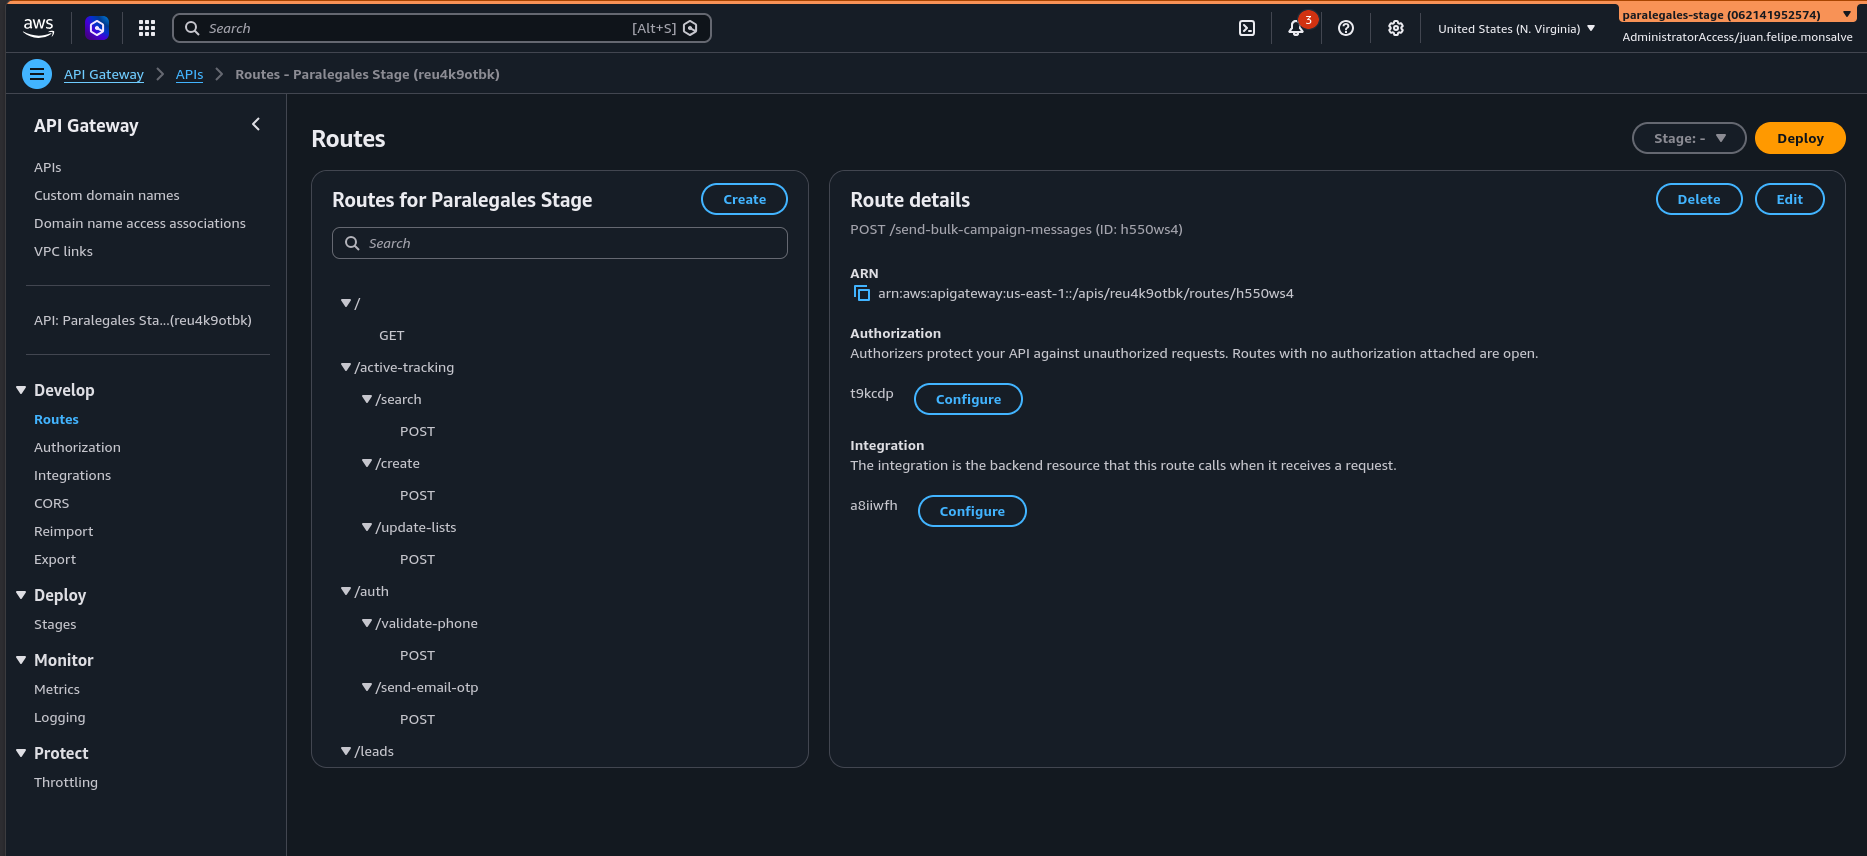
\includegraphics[width=1\textwidth]{img/figures/fig14-api-gateway.png}
  \caption[\apiGatewayCaption]{\apiGatewayCaption Fuente: Elaboración propia.}
  \label{fig:api-gateway}
\end{figure}

La capa de persistencia del sistema está respaldada por Firestore, base de datos documental de Firebase. Tal como ilustra la \autoref{fig:base-datos-firestore}, la organización de las colecciones refleja directamente los dominios de negocio de la plataforma: usuarios, procesos, seguimientos activos y planes de suscripción, entre otros. Esta estructura documental facilita la consulta eficiente de datos jerárquicos y la sincronización en tiempo real, características especialmente valiosas para los flujos reactivos implementados en el \textit{frontend}.

\newcommand\basesDatosFirestoreCaption{Estructura de colecciones y documentos en la base de datos Firestore. \hspace{1em}}
\begin{figure}[H]
  \centering
  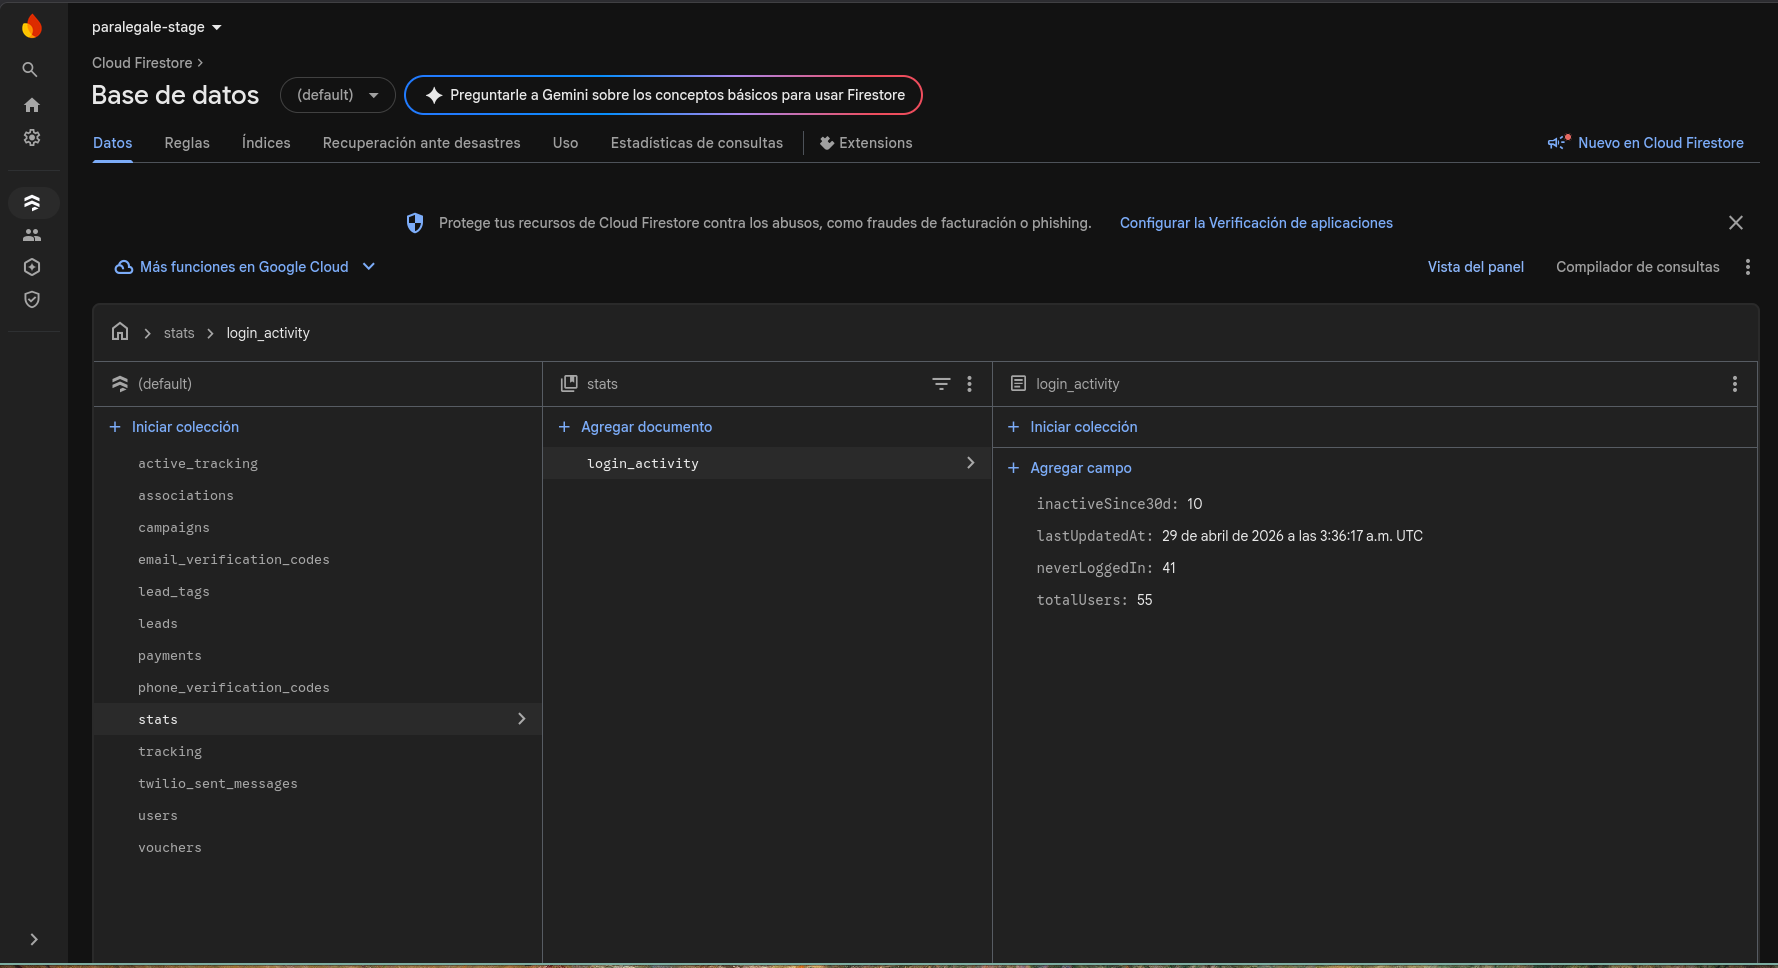
\includegraphics[width=1\textwidth]{img/figures/fig14-base-datos-firestore.png}
  \caption[\basesDatosFirestoreCaption]{\basesDatosFirestoreCaption Fuente: Elaboración propia.}
  \label{fig:base-datos-firestore}
\end{figure}

Establecidos los fundamentos tecnológicos y la organización arquitectónica del sistema, los siguientes apartados describen los módulos funcionales que dan forma a las capacidades de negocio de Paralegales, comenzando por el módulo transversal que regula el acceso a toda la plataforma: la autenticación.

\subsection{Módulo de Autenticación y Seguridad}\label{subsec:autenticacion}

El acceso seguro y controlado a la información constituye un pilar fundamental en el desarrollo de aplicaciones web de grado empresarial. Para Paralegales, se diseñó e implementó un módulo de autenticación integral que delega explícitamente la gestión de identidades a Firebase Authentication, plataforma de \textit{Backend como Servicio} (BaaS) respaldada por Google. Esta elección permitió integrar una infraestructura ya probada en materia de seguridad, encriptación y escalabilidad, reduciendo significativamente el tiempo de desarrollo sin sacrificar los estándares de protección requeridos por la plataforma.

A nivel arquitectónico, el módulo se diseñó bajo un patrón que desacopla estrictamente la lógica de negocio de la capa de presentación. Las interfaces gráficas se construyeron mediante componentes modulares y reutilizables, mientras que la interacción con el SDK de Firebase se abstrajo en capas lógicas independientes. Esta separación previene condiciones de carrera durante los tiempos de carga y permite que la aplicación cliente interactúe de manera estructurada con Firestore para sincronizar la información del perfil del usuario tras una autenticación exitosa.

\subsubsection{Funcionalidades de Autenticación y Gestión de Cuenta}

El sistema ofrece múltiples mecanismos de acceso y autogestión que equilibran la seguridad técnica con la fluidez en la experiencia de usuario:

\begin{itemize}
  \item \textbf{Registro e inicio de sesión tradicional:} se implementó un flujo estándar de creación de cuentas y acceso mediante correo electrónico y contraseña. Durante el registro, la aplicación realiza validaciones exhaustivas en tiempo real y, una vez autorizada la petición, orquesta la creación del perfil inicial del usuario en la base de datos. En el inicio de sesión, el sistema evalúa activamente el estado de la cuenta, bloqueando el acceso a funcionalidades internas si la identidad aún no ha sido confirmada.

  \item \textbf{Autenticación de terceros (SSO con Google):} para reducir la fricción en el proceso de registro, se integró el inicio de sesión único (\textit{Single Sign-On}, SSO) utilizando la infraestructura de Google. Este mecanismo incluye una lógica condicional que determina dinámicamente si el correo corresponde a un usuario nuevo o existente, previniendo la duplicación de perfiles y garantizando la integridad de los datos.
\end{itemize}

Las interfaces de inicio de sesión y registro, ilustradas en la \autoref{fig:login-screen} y la \autoref{fig:register-screen} respectivamente, presentan formularios con validación reactiva que orientan al usuario en tiempo real ante errores de entrada. La \autoref{fig:sso-google} muestra el flujo de autenticación mediante Google, que permite acceder a la plataforma en un único paso sin necesidad de gestionar credenciales adicionales.

\newcommand\loginScreenCaption{Pantalla de inicio de sesión de la plataforma Paralegales. \hspace{1em}}
\begin{figure}[H]
  \centering
  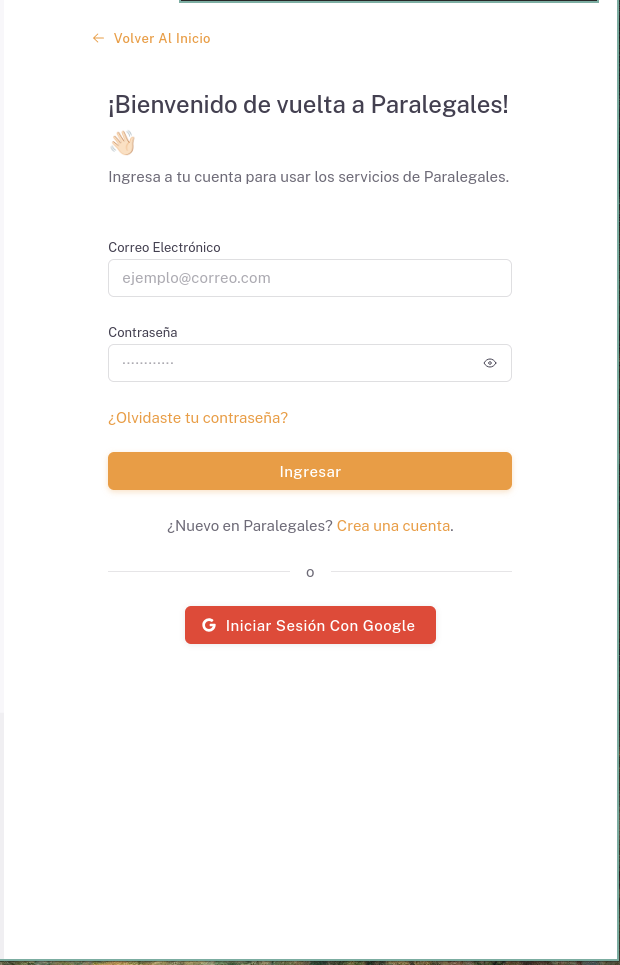
\includegraphics[width=0.85\textwidth]{img/figures/fig15-login.png}
  \caption[\loginScreenCaption]{\loginScreenCaption Fuente: Elaboración propia.}
  \label{fig:login-screen}
\end{figure}

\newcommand\registerScreenCaption{Pantalla de registro de nuevos usuarios con validación reactiva en tiempo real. \hspace{1em}}
\begin{figure}[H]
  \centering
  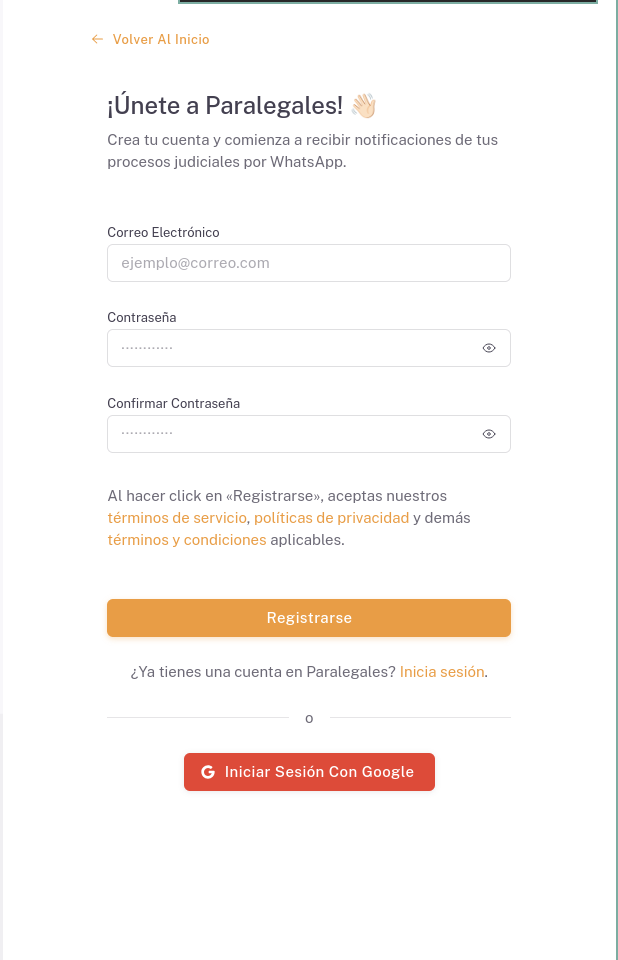
\includegraphics[width=0.85\textwidth]{img/figures/fig16-register.png}
  \caption[\registerScreenCaption]{\registerScreenCaption Fuente: Elaboración propia.}
  \label{fig:register-screen}
\end{figure}

\newcommand\ssoGoogleCaption{Flujo de autenticación mediante inicio de sesión único (SSO) con Google. \hspace{1em}}
\begin{figure}[H]
  \centering
  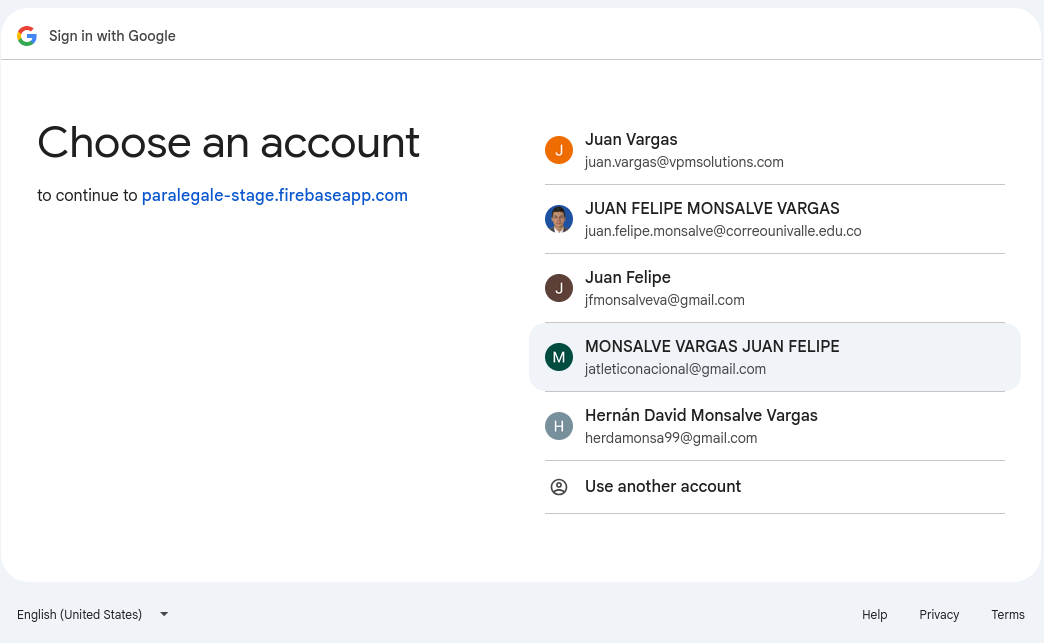
\includegraphics[width=1\textwidth]{img/figures/fig17-sso-google.png}
  \caption[\ssoGoogleCaption]{\ssoGoogleCaption Fuente: Elaboración propia.}
  \label{fig:sso-google}
\end{figure}

\begin{itemize}
  \item \textbf{Verificación de identidad por correo electrónico:} como política de seguridad para prevenir la proliferación de cuentas fraudulentas, se estableció como requisito obligatorio la validación de las direcciones de correo electrónico antes de habilitar el acceso total a la plataforma.

  \item \textbf{Recuperación de contraseña:} se incorporó un mecanismo seguro para el restablecimiento de credenciales de acceso. En caso de olvido, el usuario puede solicitar un enlace de recuperación enviado a su correo electrónico verificado, permitiendo retomar el control de la cuenta de manera autónoma y segura sin requerir intervención administrativa.
\end{itemize}

El proceso de verificación de identidad consta de dos pasos complementarios que se ilustran en las figuras \autoref{fig:email-verification-step} y \autoref{fig:email-verification-email}. En primer lugar, la plataforma informa al usuario sobre el requisito de validación y lo invita a revisar su bandeja de entrada; a continuación, el sistema envía un correo electrónico con el enlace de confirmación, bloqueando el acceso completo hasta que dicha acción sea completada.

\newcommand\emailVerificationStepCaption{Pantalla informativa del proceso de verificación de correo electrónico. \hspace{1em}}
\begin{figure}[H]
  \centering
  
\includegraphics[width=0.85\textwidth]{img/figures/fig18-email-verification-step.png}
  \caption[\emailVerificationStepCaption]{\emailVerificationStepCaption Fuente: Elaboración propia.}
  \label{fig:email-verification-step}
\end{figure}

\newcommand\emailVerificationEmailCaption{Correo electrónico de verificación de identidad enviado al usuario tras el registro. \hspace{1em}}
\begin{figure}[H]
  \centering
  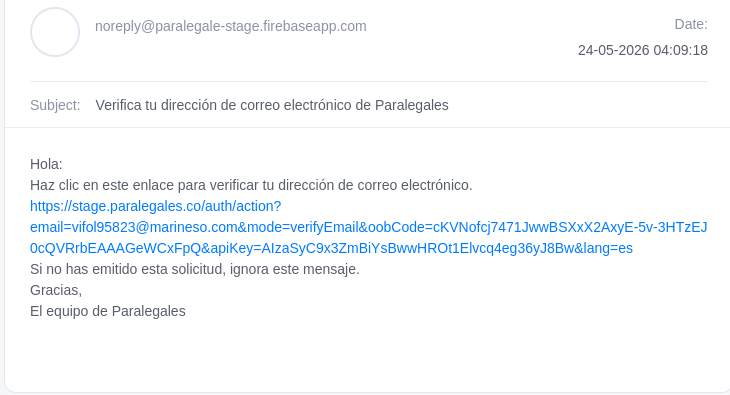
\includegraphics[width=0.65\textwidth]{img/figures/fig19-email-verification-email.png}
  \caption[\emailVerificationEmailCaption]{\emailVerificationEmailCaption Fuente: Elaboración propia.}
  \label{fig:email-verification-email}
\end{figure}

\begin{itemize}
  \item \textbf{Gestión y actualización de seguridad:} desde el panel de preferencias del perfil, los usuarios pueden gestionar directamente la seguridad de su cuenta. Se desarrollaron funcionalidades específicas para la actualización del correo electrónico y la modificación de contraseñas. Estas operaciones incorporan validaciones adicionales de protección, como la exigencia de la contraseña actual para confirmar cambios críticos, al tiempo que el sistema identifica y maneja inteligentemente el estado de los usuarios autenticados vía proveedores externos (SSO), adaptando la interfaz según corresponda.
\end{itemize}

Como se observa en la \autoref{fig:update-email-password}, la vista de seguridad del perfil unifica en una sola pantalla las opciones de actualización de correo y contraseña, adaptando su presentación según el proveedor de autenticación del usuario: los registros por SSO omiten los campos de contraseña, dado que la gestión de credenciales recae exclusivamente en el proveedor externo.

\newcommand\updateEmailPasswordCaption{Vista de gestión de seguridad de la cuenta con opciones de actualización de correo y contraseña. \hspace{1em}}
\begin{figure}[H]
  \centering
  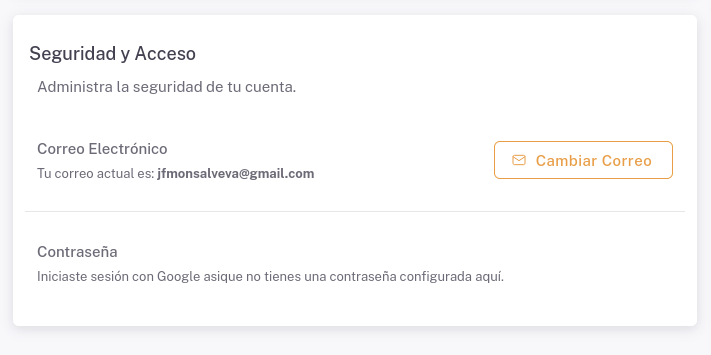
\includegraphics[width=1\textwidth]{img/figures/fig21-update-email-password-feature.png}
  \caption[\updateEmailPasswordCaption]{\updateEmailPasswordCaption Fuente: Elaboración propia.}
  \label{fig:update-email-password}
\end{figure}

\subsubsection{Interfaz Gráfica, Experiencia de Usuario y Onboarding}

El diseño visual del módulo se fundamenta en interfaces dinámicas que se adaptan al contexto del usuario. En lugar de crear vistas aisladas para cada flujo, se desarrolló un sistema de enrutamiento y componentes que consolida los diversos formularios en entornos visuales cohesivos, optimizando la navegación y reduciendo la carga cognitiva. Todo el proceso está acompañado por un manejo global de excepciones y mensajes de retroalimentación que guían al usuario de manera oportuna ante eventualidades, como interrupciones de red o uso de credenciales incorrectas.

Con el objetivo de enriquecer y personalizar la experiencia desde el primer ingreso a la plataforma, se diseñó e implementó un flujo de inicialización progresiva (\textit{onboarding}). Tras un registro exitoso, el sistema despliega una encuesta dinámica orientada a la perfilación del usuario, capturando datos profesionales relevantes tales como su nivel de especialidad legal, su profesión base y sus años de experiencia. Esta estructura de datos se somete a validación de esquemas en el entorno cliente para luego sincronizarse de manera inmediata con Firestore, lo que permite a la aplicación adaptar su funcionalidad a las necesidades particulares de cada cuenta. La \autoref{fig:onboarding} presenta el flujo de encuesta implementado, donde cada paso conduce al usuario a través de preguntas progresivas hasta completar su perfil inicial.

\newcommand\onboardingCaption{Flujo de \textit{onboarding} para la perfilación del usuario tras el registro. \hspace{1em}}
\begin{figure}[H]
  \centering
  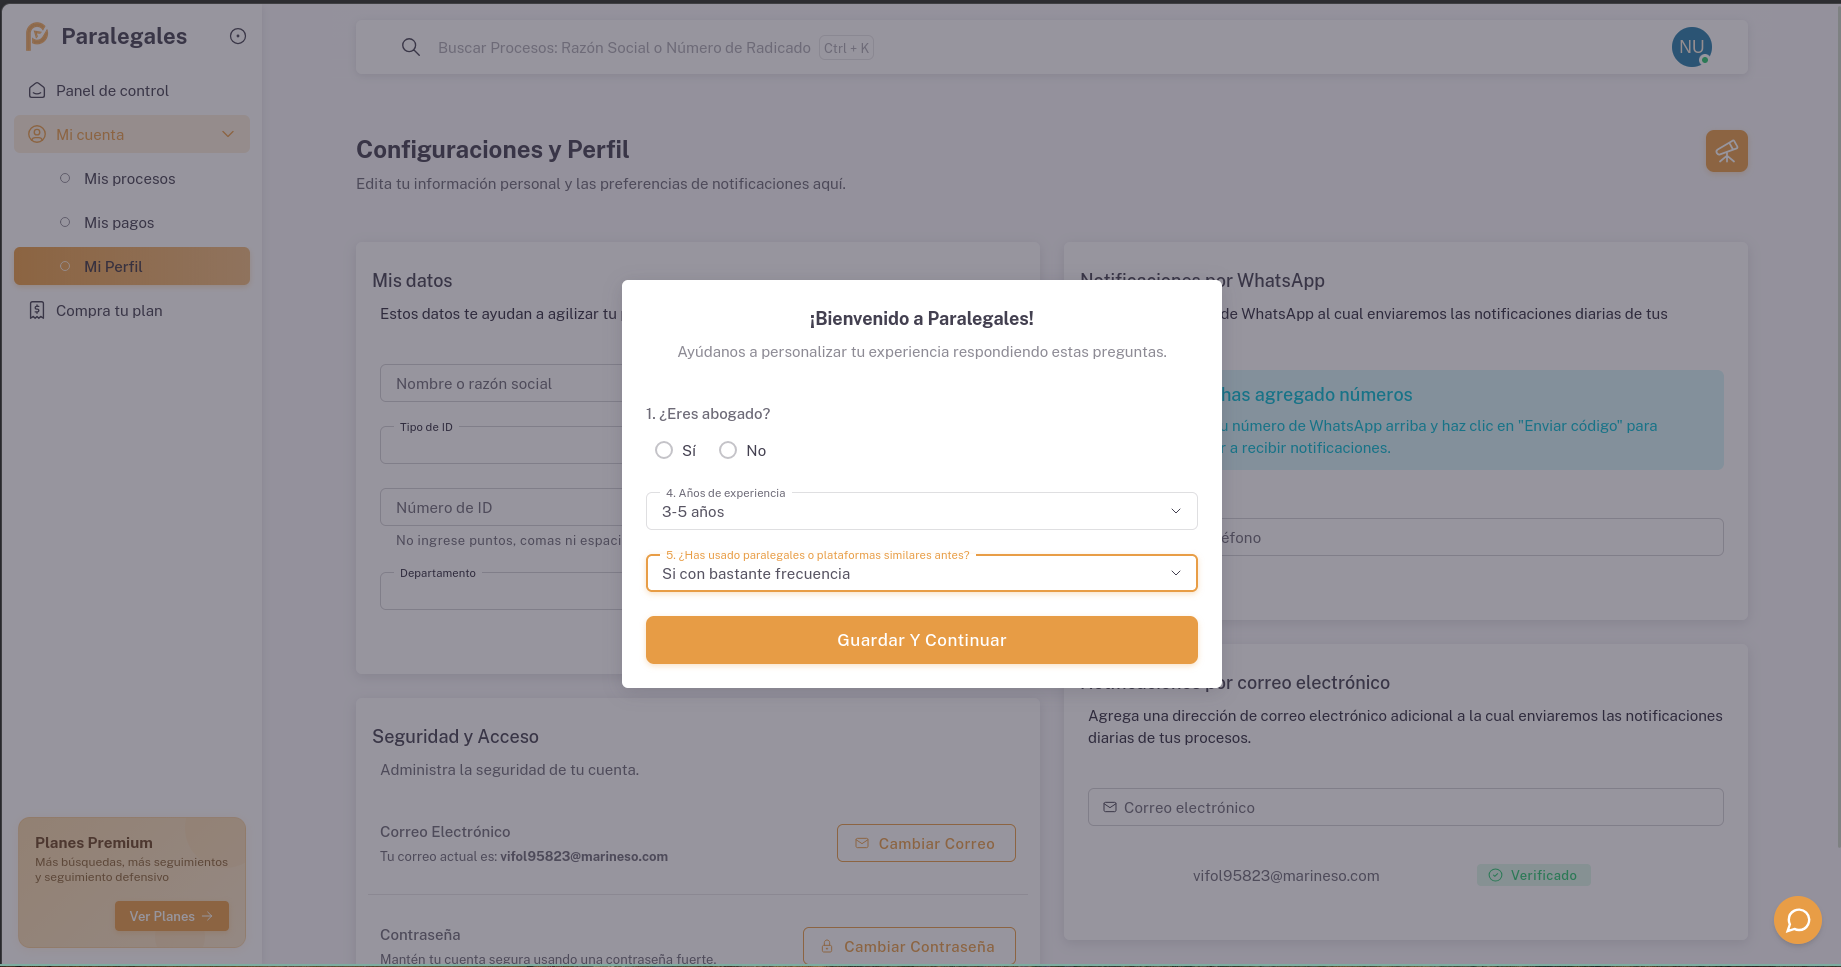
\includegraphics[width=1\textwidth]{img/figures/fig20-onboarding.png}
  \caption[\onboardingCaption]{\onboardingCaption Fuente: Elaboración propia.}
  \label{fig:onboarding}
\end{figure}

\subsubsection{Reglas de Seguridad y Control de Acceso a la Base de Datos}

De manera complementaria a la autenticación en el entorno cliente, se diseñaron e implementaron las Reglas de Seguridad de Firestore. Estas reglas son políticas declarativas que se evalúan y ejecutan directamente en los servidores de la base de datos antes de permitir cualquier operación de lectura o escritura, constituyendo la última y más robusta línea de defensa contra accesos no autorizados. Su implementación garantiza que los usuarios únicamente puedan interactuar con la información que les pertenece o sobre la que tienen permisos explícitos.

Dado que el control de acceso a los documentos representa una de las partes más críticas del sistema, el diseño de estas reglas estuvo respaldado por una batería de pruebas unitarias automatizadas. La inclusión de estos \textit{tests} permitió verificar de forma rigurosa cada política de acceso frente a múltiples escenarios y simulaciones de ataque, asegurando que ninguna brecha de seguridad comprometiera la privacidad ni la integridad de la información almacenada. La \autoref{fig:security-rules-firebase} ilustra el conjunto de reglas de seguridad implementadas sobre las colecciones principales de Firestore, donde cada documento está protegido mediante condiciones explícitas que validan la identidad del solicitante antes de autorizar cualquier operación. Una vez garantizado el control de identidad como cimiento transversal del sistema, el siguiente módulo entrega el valor central de la plataforma: la consulta, el seguimiento y la gestión de procesos judiciales.

\newcommand\securityRulesFirebaseCaption{Reglas de seguridad de Firestore que controlan el acceso a las colecciones de la plataforma. \hspace{1em}}
\begin{figure}[H]
  \centering
  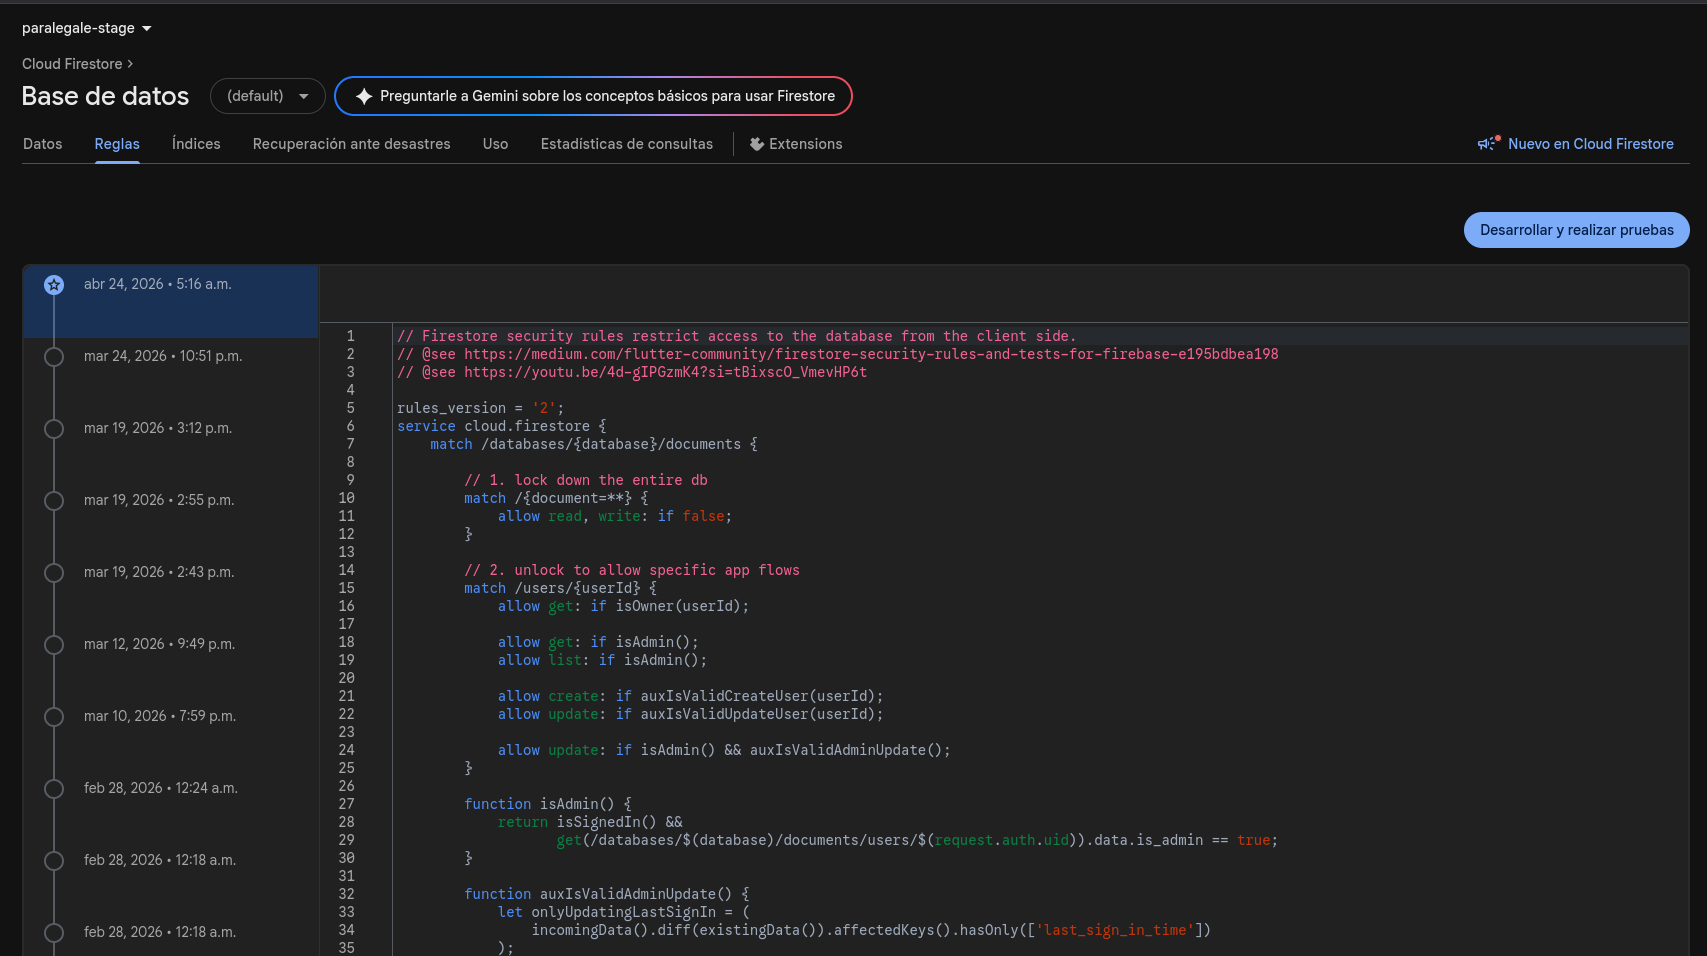
\includegraphics[width=1\textwidth]{img/figures/fig22-security-rules-in-firebase.png}
  \caption[\securityRulesFirebaseCaption]{\securityRulesFirebaseCaption Fuente: Elaboración propia.}
  \label{fig:security-rules-firebase}
\end{figure}

\subsection{Módulo de Procesos}\label{subsec:procesos}

El Módulo de Procesos constituye el núcleo operativo de la plataforma, dotando a los usuarios de las herramientas necesarias para la búsqueda, vinculación y gestión de los procesos judiciales de su interés. Su desarrollo abarca desde herramientas para la consulta manual y un panel de control centralizado, hasta capacidades de automatización mediante el monitoreo constante de expedientes. Todo esto involucró la creación de interfaces de usuario interactivas, la integración con servicios externos de información jurídica y la construcción de una sólida capa de comunicación con el \textit{backend} del sistema.

\subsubsection{Panel de Control Centralizado (Dashboard)}

Para ofrecer una experiencia de usuario eficiente y reducir la fricción operativa, se desarrolló una vista principal (\textit{Dashboard}) que actúa como el punto de entrada para el usuario autenticado. Esta interfaz fue diseñada bajo un enfoque de modularidad, componiéndose de diversas tarjetas y \textit{widgets} interactivos que consolidan la información más relevante de la cuenta. A través de este panel, el usuario obtiene una visión panorámica e inmediata de sus estadísticas generales, el estado de sus planes activos y el acceso directo a sus procesos judiciales más recientes, facilitando la toma de decisiones y permitiendo ejecutar acciones rápidas sin la necesidad de navegar profundamente por las distintas secciones de la plataforma. La \autoref{fig:dashboard-procesos} muestra el \textit{dashboard} principal con sus componentes de resumen, estadísticas y accesos directos organizados en una cuadrícula adaptativa.

\newcommand\dashboardProcesosCaption{\textit{Dashboard} principal del módulo de procesos con estadísticas y accesos directos al usuario. \hspace{1em}}
\begin{figure}[H]
  \centering
  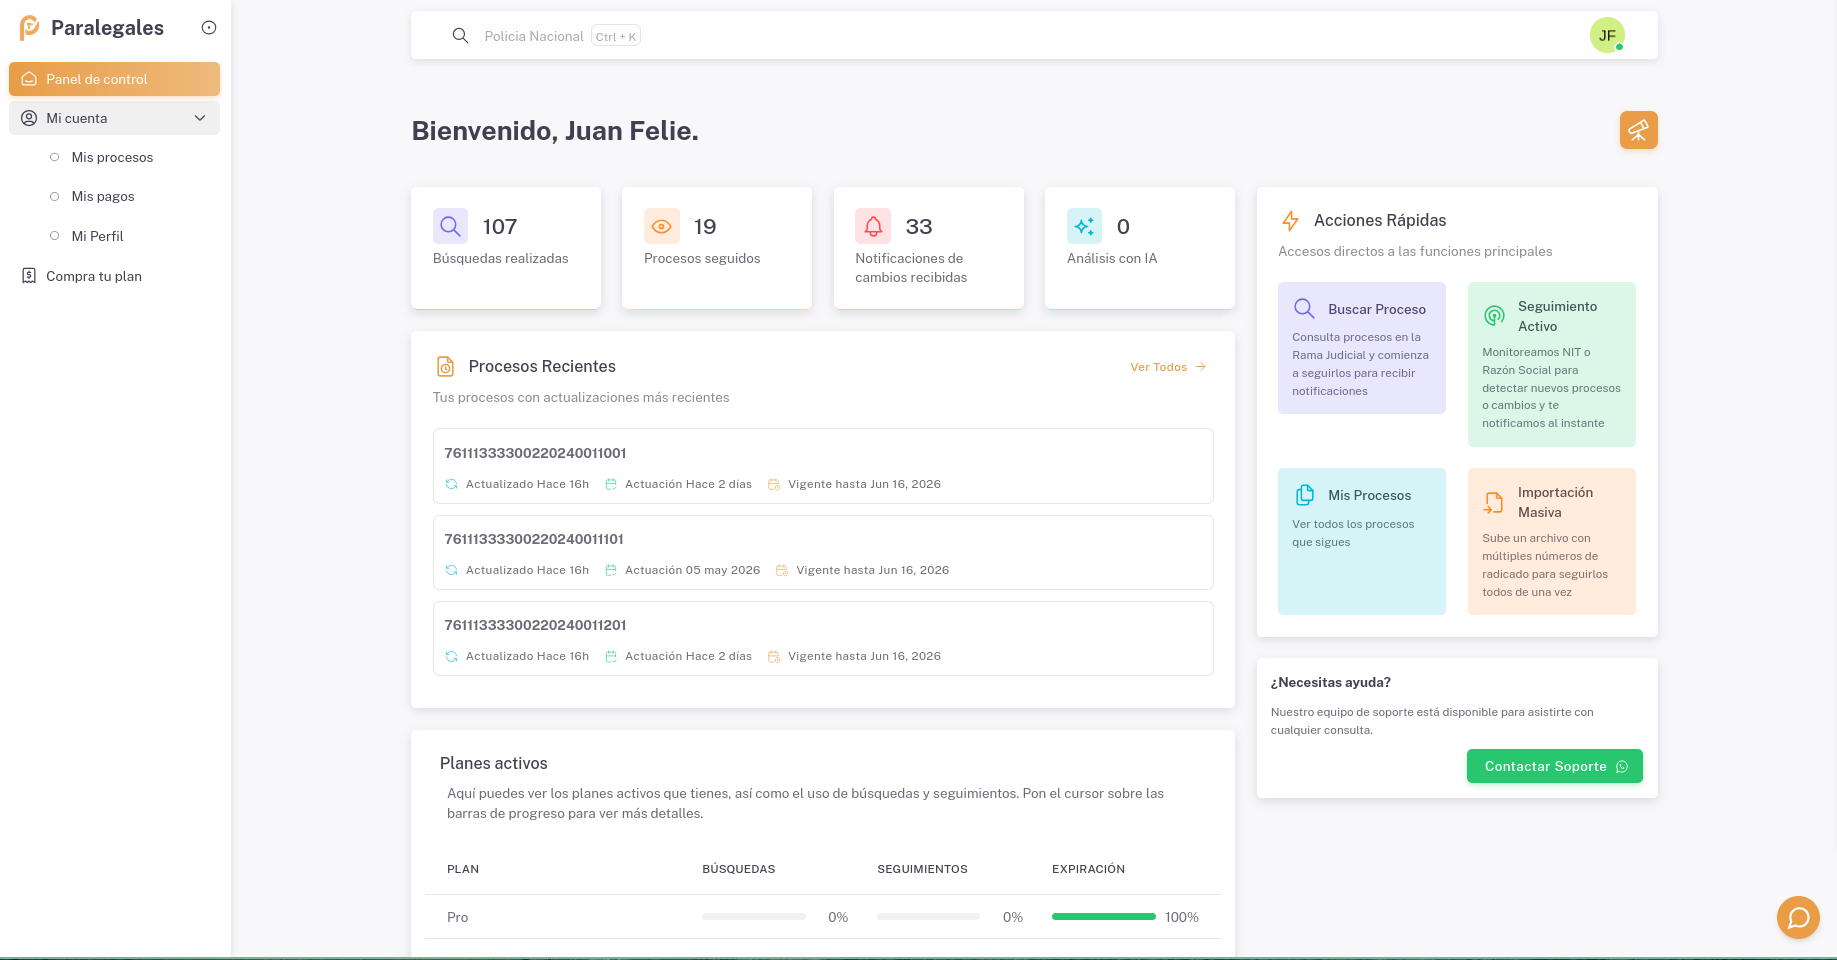
\includegraphics[width=1\textwidth]{img/figures/fig23-dashboard-procesos.png}
  \caption[\dashboardProcesosCaption]{\dashboardProcesosCaption Fuente: Elaboración propia.}
  \label{fig:dashboard-procesos}
\end{figure}

\subsubsection{Búsqueda de Procesos e Integración con la Rama Judicial}

Uno de los requerimientos más críticos de la plataforma fue proveer un motor de búsqueda que permitiera consultar procesos directamente desde las bases de datos de la Rama Judicial. Dado que la entidad proporciona un portal público pero carece de una API documentada y orientada a desarrolladores, se llevó a cabo un proceso de ingeniería inversa que consistió en interceptar, analizar y mapear el tráfico de red generado por el portal oficial durante consultas legítimas. A través de este análisis, se identificaron los distintos \textit{endpoints} utilizados por la entidad y la estructura de los \textit{payloads} requeridos, abarcando desde las consultas de parametrización (departamentos, ciudades, especialidades y entidades) hasta las búsquedas directas por código de radicado o nombre del implicado.

Para la integración a nivel de software, se diseñó una arquitectura de \textit{proxy} en el servidor de la aplicación. En lugar de que el \textit{frontend} realizara las peticiones directamente a los servidores gubernamentales, estas se encapsularon en una capa de servicios intermediarios dentro del BFF. Esta decisión arquitectónica aportó múltiples beneficios: permitió superar las restricciones de políticas de mismo origen (CORS), estandarizó los esquemas de respuesta hacia las vistas de la aplicación, y habilitó la incorporación de capas de observabilidad, manejo de errores centralizado y generación de \textit{logs} de auditoría. En el \textit{frontend}, las vistas de resultados consumen esta API interna de forma segura y estructurada, presentando la información judicial al usuario de manera clara y eficiente.

La \autoref{fig:filtros-busqueda-procesos} expone el formulario de búsqueda avanzada, donde el usuario puede combinar múltiples criterios de filtrado —como departamento, ciudad, especialidad y entidad— para acotar el universo de expedientes consultados. La \autoref{fig:resultados-busqueda} ilustra la vista de resultados que despliega la lista de procesos encontrados, con la información relevante de cada expediente organizada de forma tabular y con indicadores de estado claramente diferenciados.

\newcommand\filtrosBusquedaProcesosCaption{Formulario de búsqueda avanzada de procesos judiciales con filtros combinables. \hspace{1em}}
\begin{figure}[H]
  \centering
  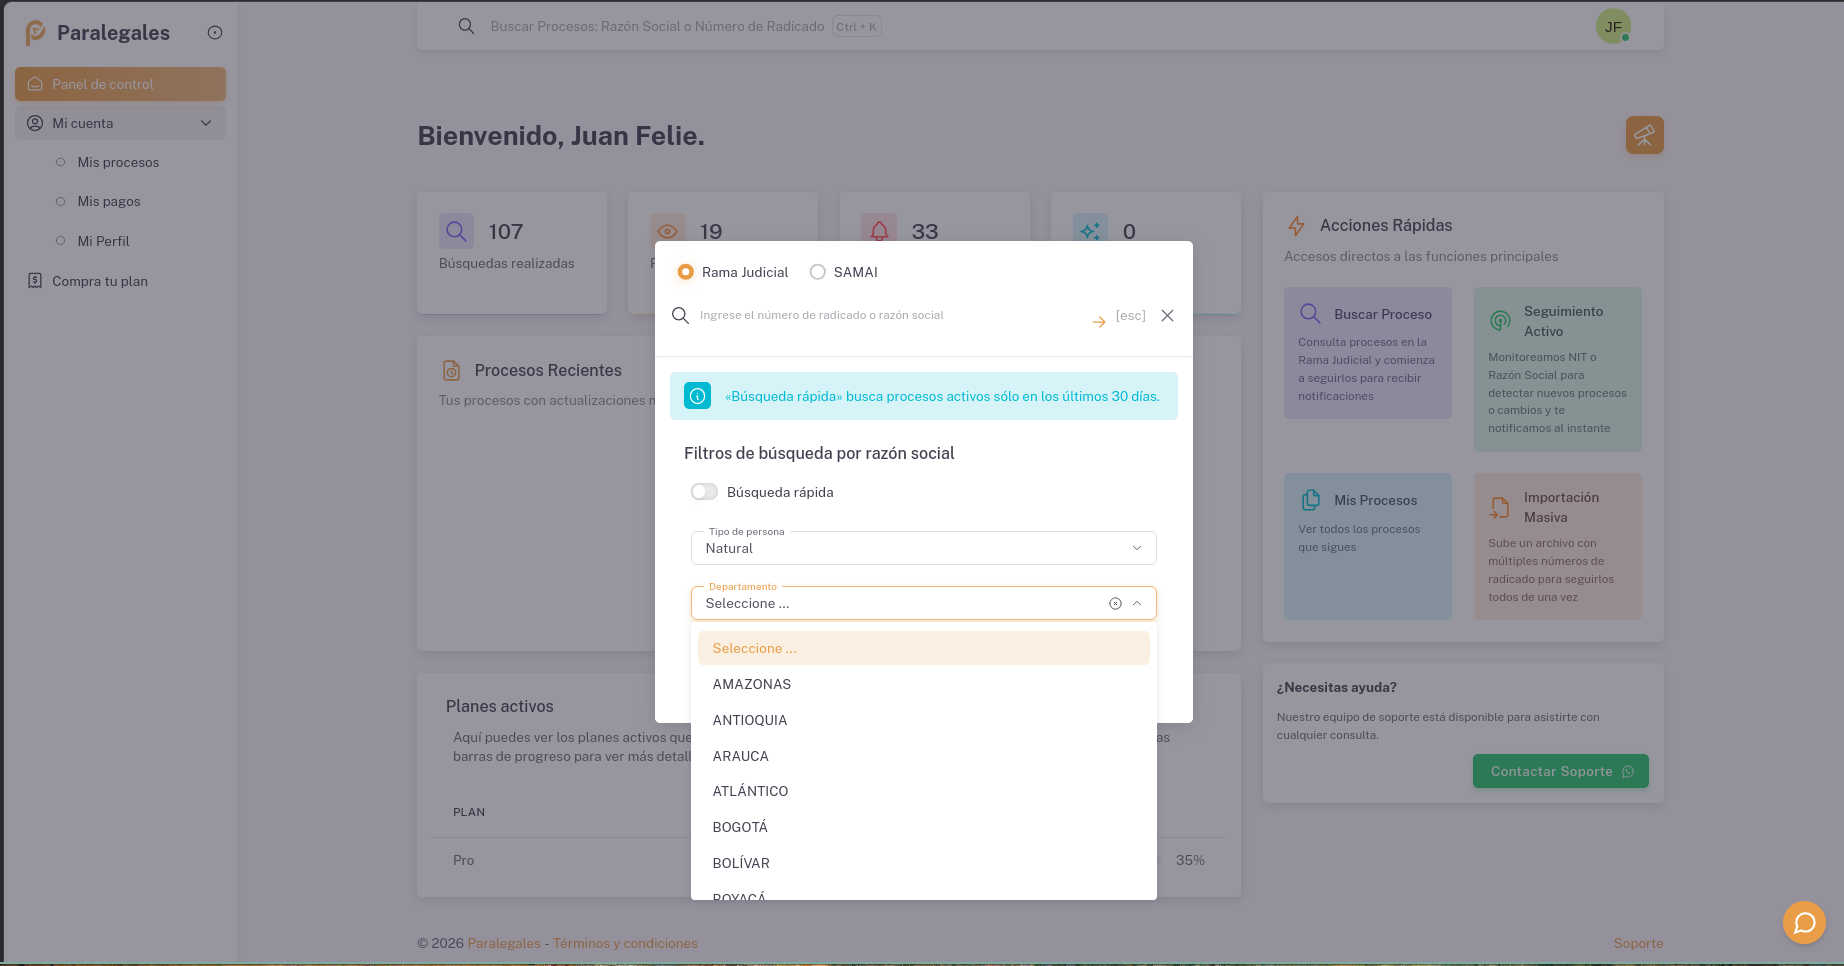
\includegraphics[width=1\textwidth]{img/figures/fig24-filtros-busquedas-procesos.png}
  \caption[\filtrosBusquedaProcesosCaption]{\filtrosBusquedaProcesosCaption Fuente: Elaboración propia.}
  \label{fig:filtros-busqueda-procesos}
\end{figure}

\newcommand\resultadosBusquedaCaption{Vista de resultados de la búsqueda de procesos judiciales en la Rama Judicial. \hspace{1em}}
\begin{figure}[H]
  \centering
  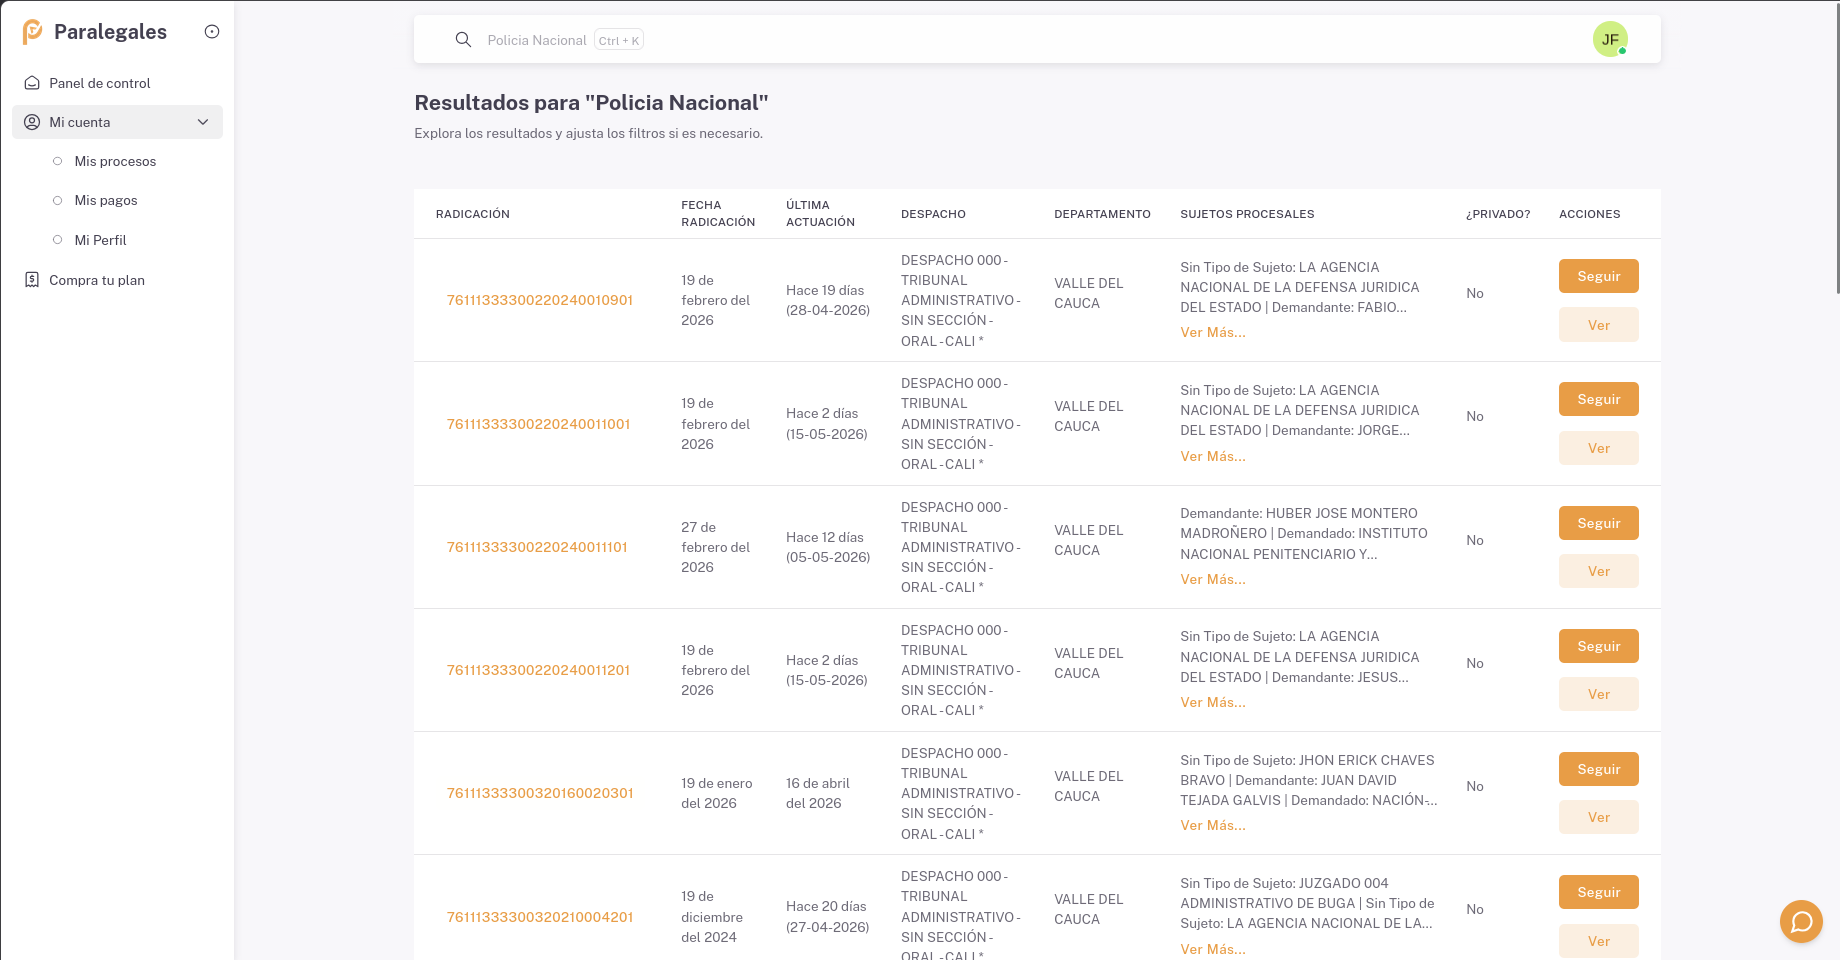
\includegraphics[width=1\textwidth]{img/figures/fig25-results-process.png}
  \caption[\resultadosBusquedaCaption]{\resultadosBusquedaCaption Fuente: Elaboración propia.}
  \label{fig:resultados-busqueda}
\end{figure}

\subsubsection{Seguimiento de Procesos}

Una vez localizado un proceso a través del motor de búsqueda, el sistema le brinda al usuario la capacidad de agregarlo a su portafolio personal para un monitoreo continuo. Esta funcionalidad de seguimiento (\textit{follow}) y cancelación del mismo (\textit{unfollow}) requirió un diseño cuidadoso para garantizar una experiencia reactiva e instantánea.

En el \textit{frontend}, la implementación separa estrictamente la capa de presentación de la lógica de negocio: se desarrollaron componentes visuales atómicos y reutilizables —como botones interactivos con estados de carga— cuya lógica de interacción fue abstraída mediante \textit{composables}. Estos encapsulan el manejo del estado local, la reactividad y las excepciones, invocando a su vez repositorios dedicados a la comunicación de red. La orquestación lógica de asociar o desvincular un proceso a un usuario fue delegada y centralizada en los servicios \textit{backend}, de modo que el \textit{frontend} solo emite la intención del usuario y reacciona al resultado actualizando la interfaz de forma instantánea. La \autoref{fig:follow-process} presenta el componente de acción de seguimiento integrado en la vista de resultados, donde el usuario puede vincular un expediente a su cuenta mediante una única interacción.

\newcommand\followProcessCaption{Componente de seguimiento de proceso judicial accesible desde la vista de resultados de búsqueda. \hspace{1em}}
\begin{figure}[H]
  \centering
  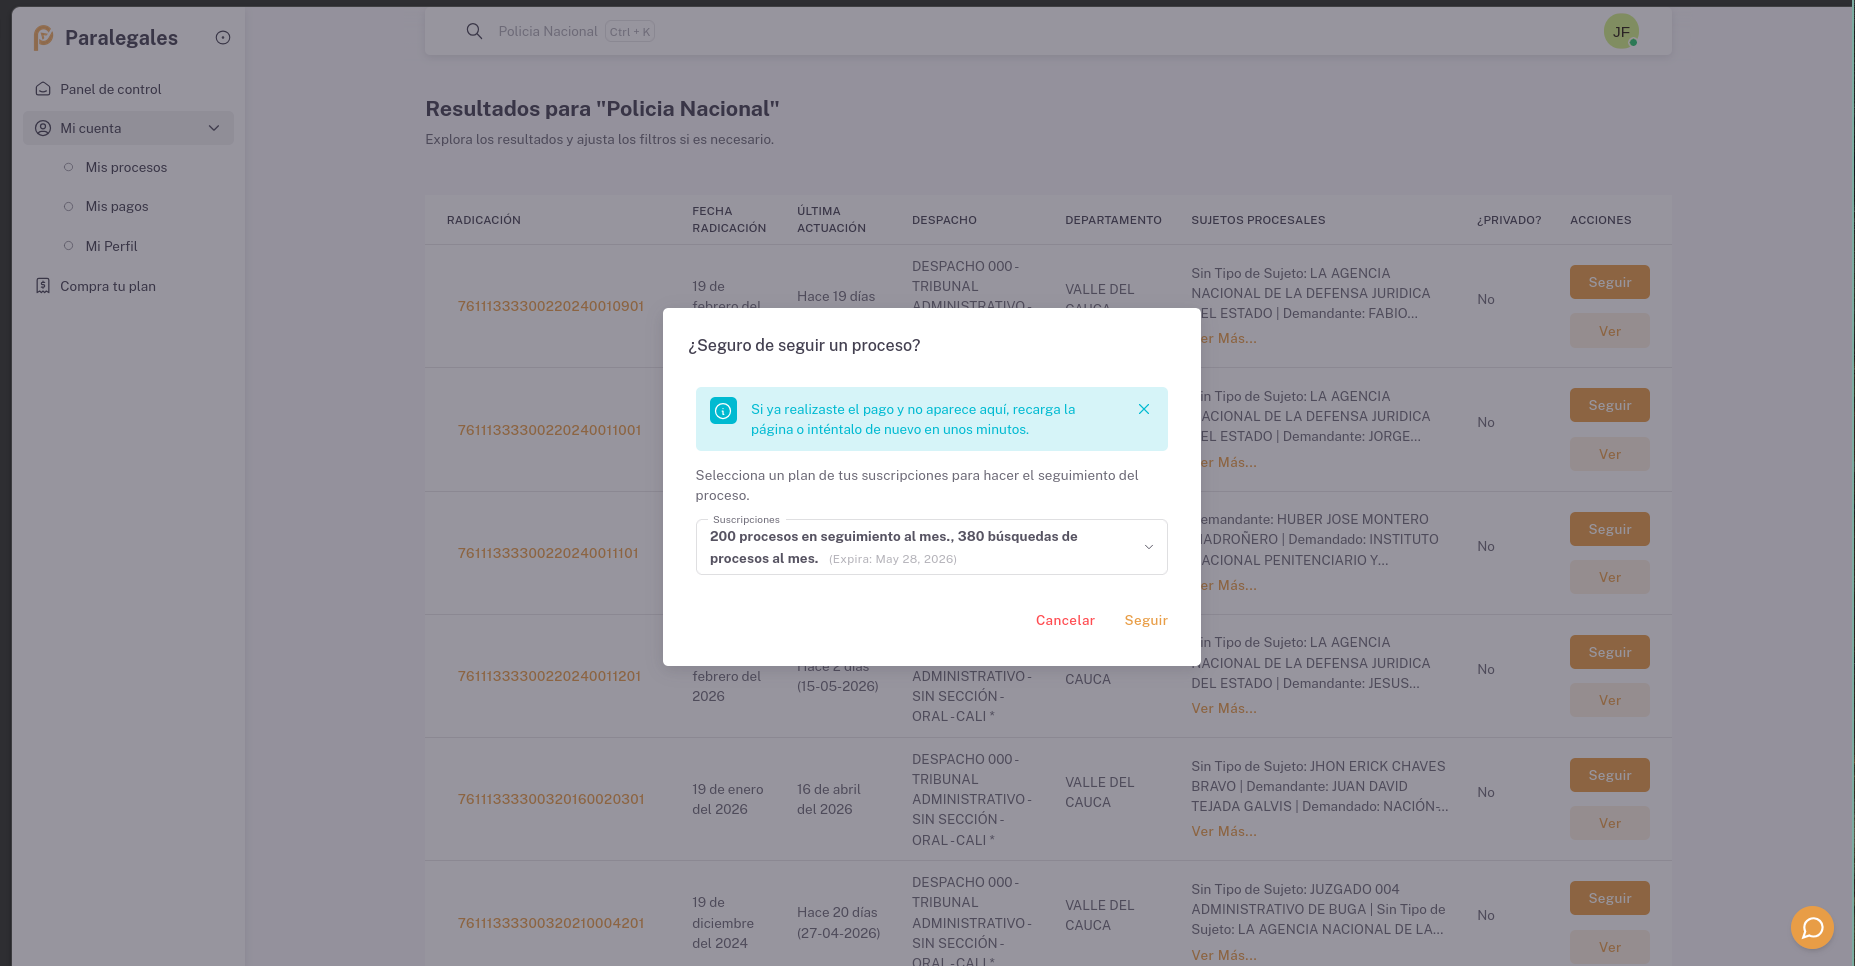
\includegraphics[width=1\textwidth]{img/figures/fig26-follow-process.png}
  \caption[\followProcessCaption]{\followProcessCaption Fuente: Elaboración propia.}
  \label{fig:follow-process}
\end{figure}

\subsubsection{Gestión y Visualización: Mis Procesos}

Para centralizar la información de cada usuario, se desarrolló la vista ``Mis Procesos'', que actúa como el panel de control personal del usuario, listando en un formato estructurado y amigable todos los procesos bajo seguimiento activo.

El diseño de esta vista se enfocó en la modularidad y el rendimiento. La interfaz recupera de manera asíncrona la lista de procesos vinculados al usuario autenticado a través de la interacción entre el cliente y el \textit{backend}. El componente es altamente reactivo: si el usuario decide cancelar el seguimiento de un proceso desde este panel, el sistema invoca la abstracción de seguimiento descrita anteriormente y el proceso se elimina de la vista en tiempo real, sin requerir recargas de página, ofreciendo una experiencia ininterrumpida. Como se aprecia en la \autoref{fig:my-processes-view}, la vista organiza los expedientes en tarjetas con información resumida —radicado, entidad, estado y fecha de última actuación—, permitiendo al usuario identificar rápidamente los casos que requieren su atención.

\newcommand\myProcessesViewCaption{Vista ``Mis Procesos'' con la lista de expedientes bajo seguimiento activo del usuario. \hspace{1em}}
\begin{figure}[H]
  \centering
  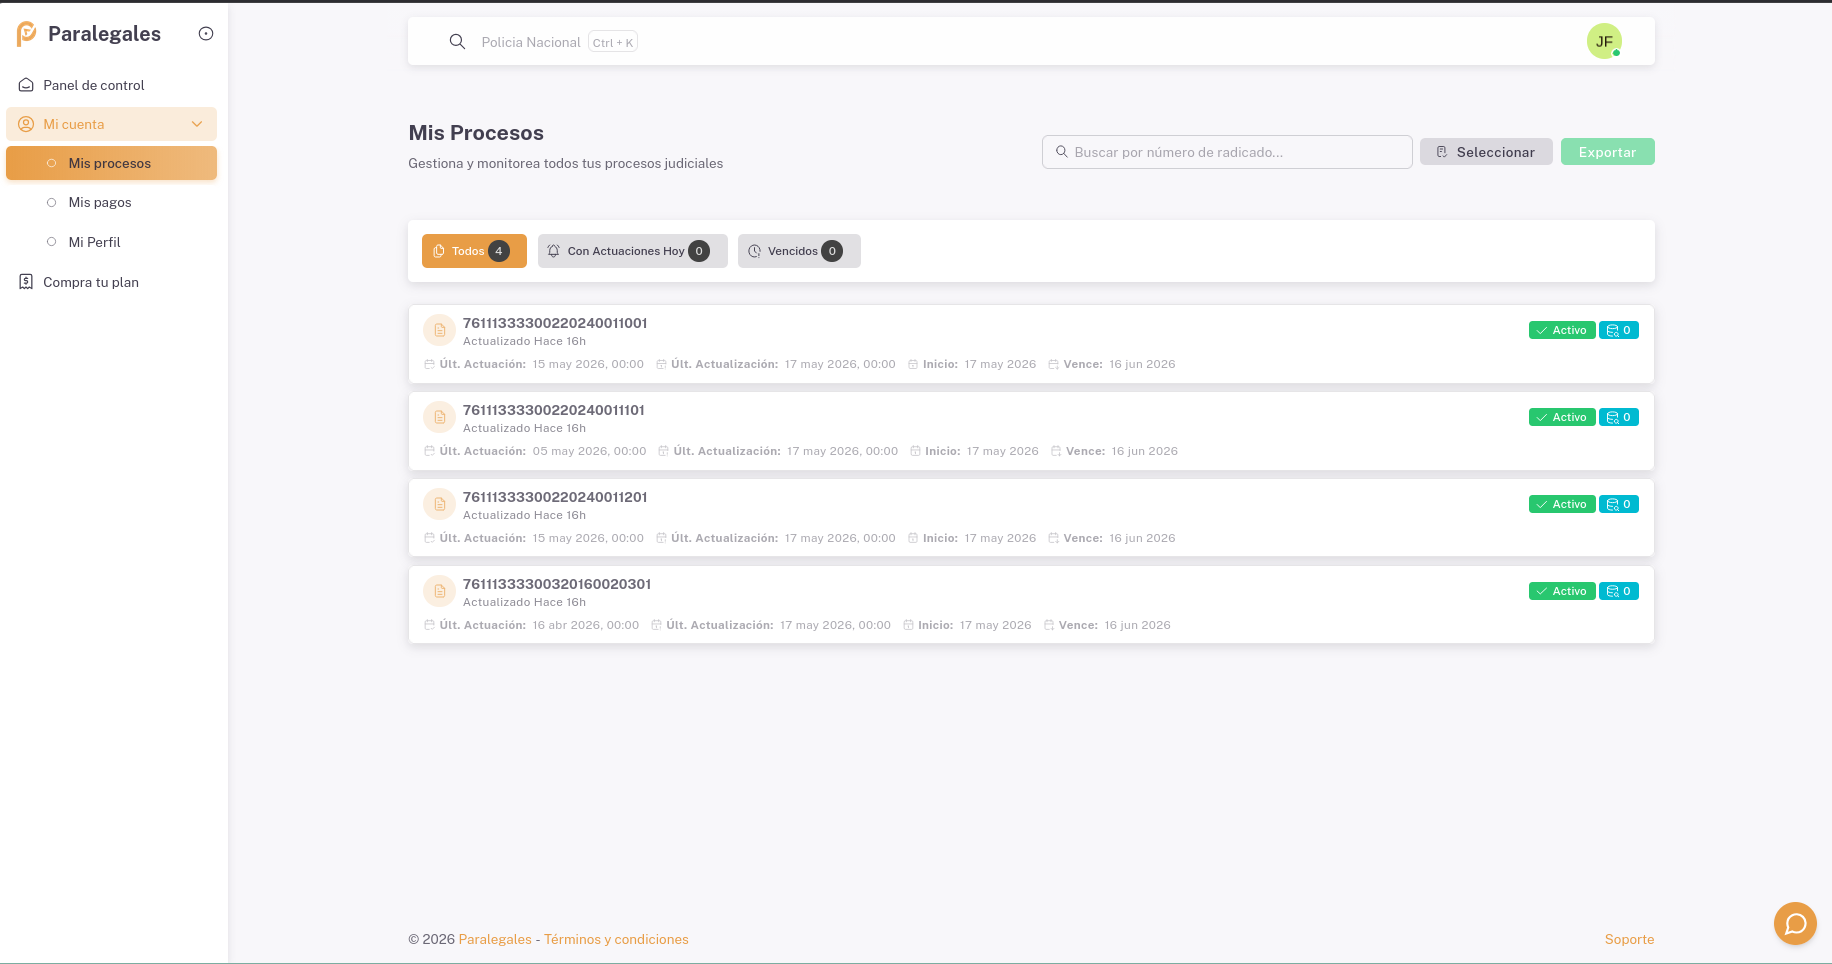
\includegraphics[width=1\textwidth]{img/figures/fig27-my-processes-view.png}
  \caption[\myProcessesViewCaption]{\myProcessesViewCaption Fuente: Elaboración propia.}
  \label{fig:my-processes-view}
\end{figure}

\subsubsection{Automatización mediante Seguimientos Activos}

Más allá del seguimiento manual, el módulo introduce un subsistema de automatización denominado ``Seguimientos Activos''. Esta funcionalidad exime al usuario de realizar consultas manuales repetitivas al delegar al sistema la búsqueda diaria de procesos judiciales asociados a un parámetro de interés, tal como un Número de Identificación Tributaria (NIT) o la Razón Social de una persona natural o jurídica.

A nivel arquitectónico en el \textit{frontend}, la lógica de negocio y las peticiones de red fueron abstraídas en funciones componibles (\textit{composables}), las cuales alimentan las interfaces de usuario de manera reactiva. La creación de un nuevo seguimiento requiere la validación y vinculación a un plan de pago o suscripción activa del usuario, integrando así los servicios operativos con el modelo de facturación. Una vez configurado, el motor de búsqueda rastrea diversas bases de datos en segundo plano, incluyendo la Rama Judicial y el sistema de información SAMAI. La \autoref{fig:seguimiento-activo} muestra el formulario de configuración de un nuevo seguimiento activo, donde el usuario define el parámetro de búsqueda y lo vincula a su plan vigente.

\newcommand\seguimientoActivoCaption{Formulario de configuración de un nuevo seguimiento activo con vinculación al plan de suscripción. \hspace{1em}}
\begin{figure}[H]
  \centering
  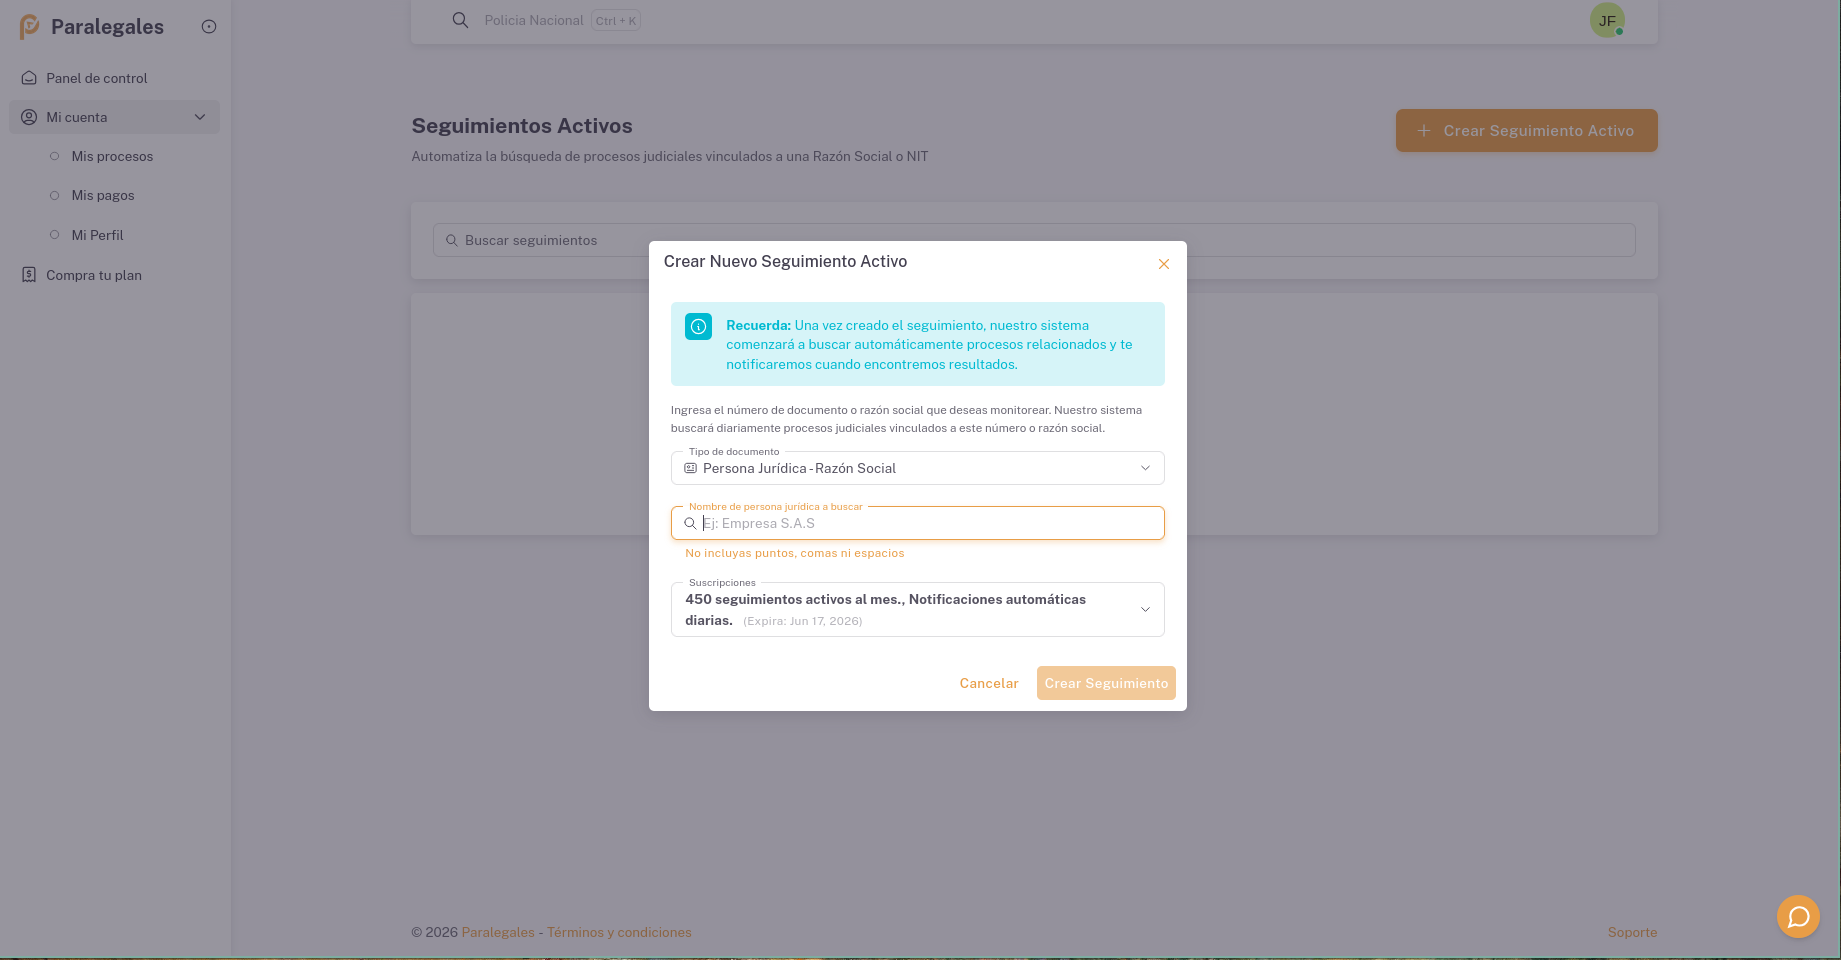
\includegraphics[width=1\textwidth]{img/figures/fig28-seguimiento-activo.png}
  \caption[\seguimientoActivoCaption]{\seguimientoActivoCaption Fuente: Elaboración propia.}
  \label{fig:seguimiento-activo}
\end{figure}

Para la revisión de los resultados, se diseñó una vista de detalle basada en pestañas que separa los ``Procesos Encontrados'' de una ``Lista Blanca''. Esta interfaz proporciona una experiencia de clasificación interactiva: el usuario puede revisar los nuevos hallazgos y decidir, mediante acciones asíncronas, si los aprueba (incorporándolos a su lista blanca) o los descarta (enviándolos a una lista negra). La \autoref{fig:seguimiento-activo-details} ilustra esta vista de detalle con los resultados organizados en pestañas, facilitando la clasificación progresiva de coincidencias. De esta manera, se garantiza un filtrado progresivo y personalizado, optimizando el tiempo invertido en la depuración de coincidencias homónimas o irrelevantes. La \autoref{fig:seguimiento-activo-success} confirma la retroalimentación visual que recibe el usuario al aprobar un proceso encontrado, reforzando la confianza en la operación completada.

\newcommand\seguimientoActivoDetailsCaption{Vista de detalle del seguimiento activo con resultados organizados en pestañas de clasificación. \hspace{1em}}
\begin{figure}[H]
  \centering
  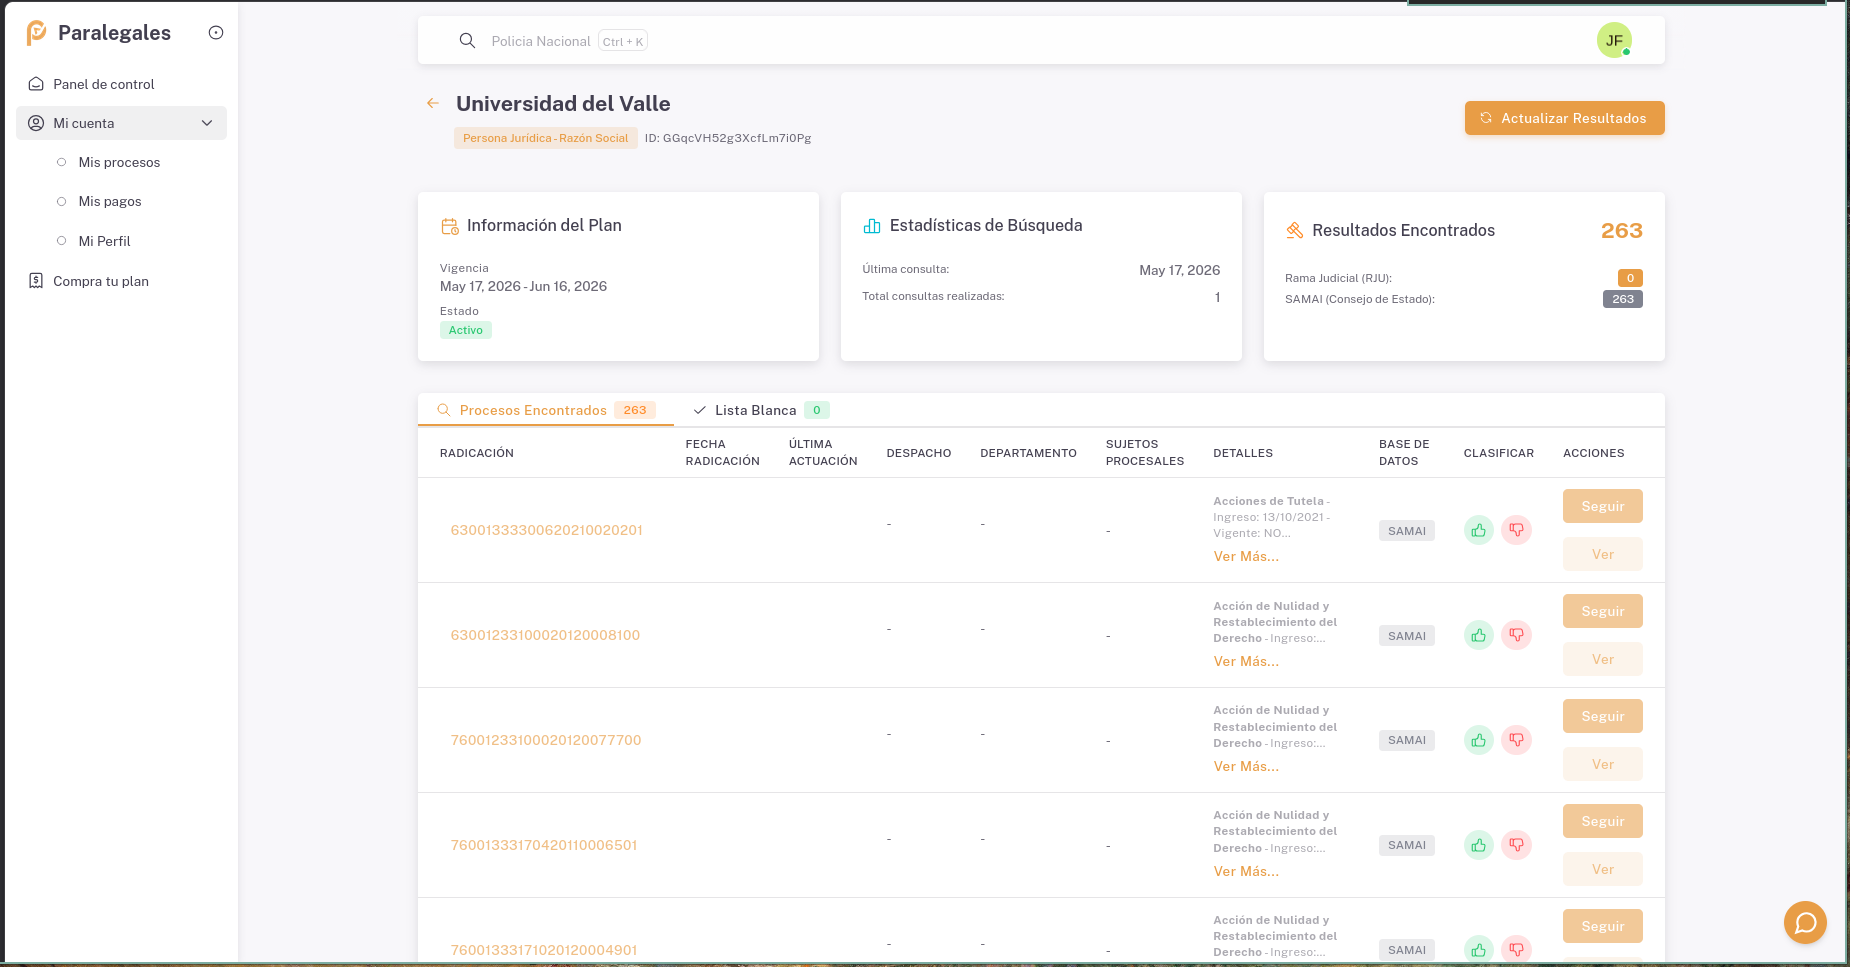
\includegraphics[width=1\textwidth]{img/figures/fig20-seguimiento-activo-details.png}
  \caption[\seguimientoActivoDetailsCaption]{\seguimientoActivoDetailsCaption Fuente: Elaboración propia.}
  \label{fig:seguimiento-activo-details}
\end{figure}

\newcommand\seguimientoActivoSuccessCaption{Confirmación visual tras la aprobación de un proceso encontrado en el seguimiento activo. \hspace{1em}}
\begin{figure}[H]
  \centering
  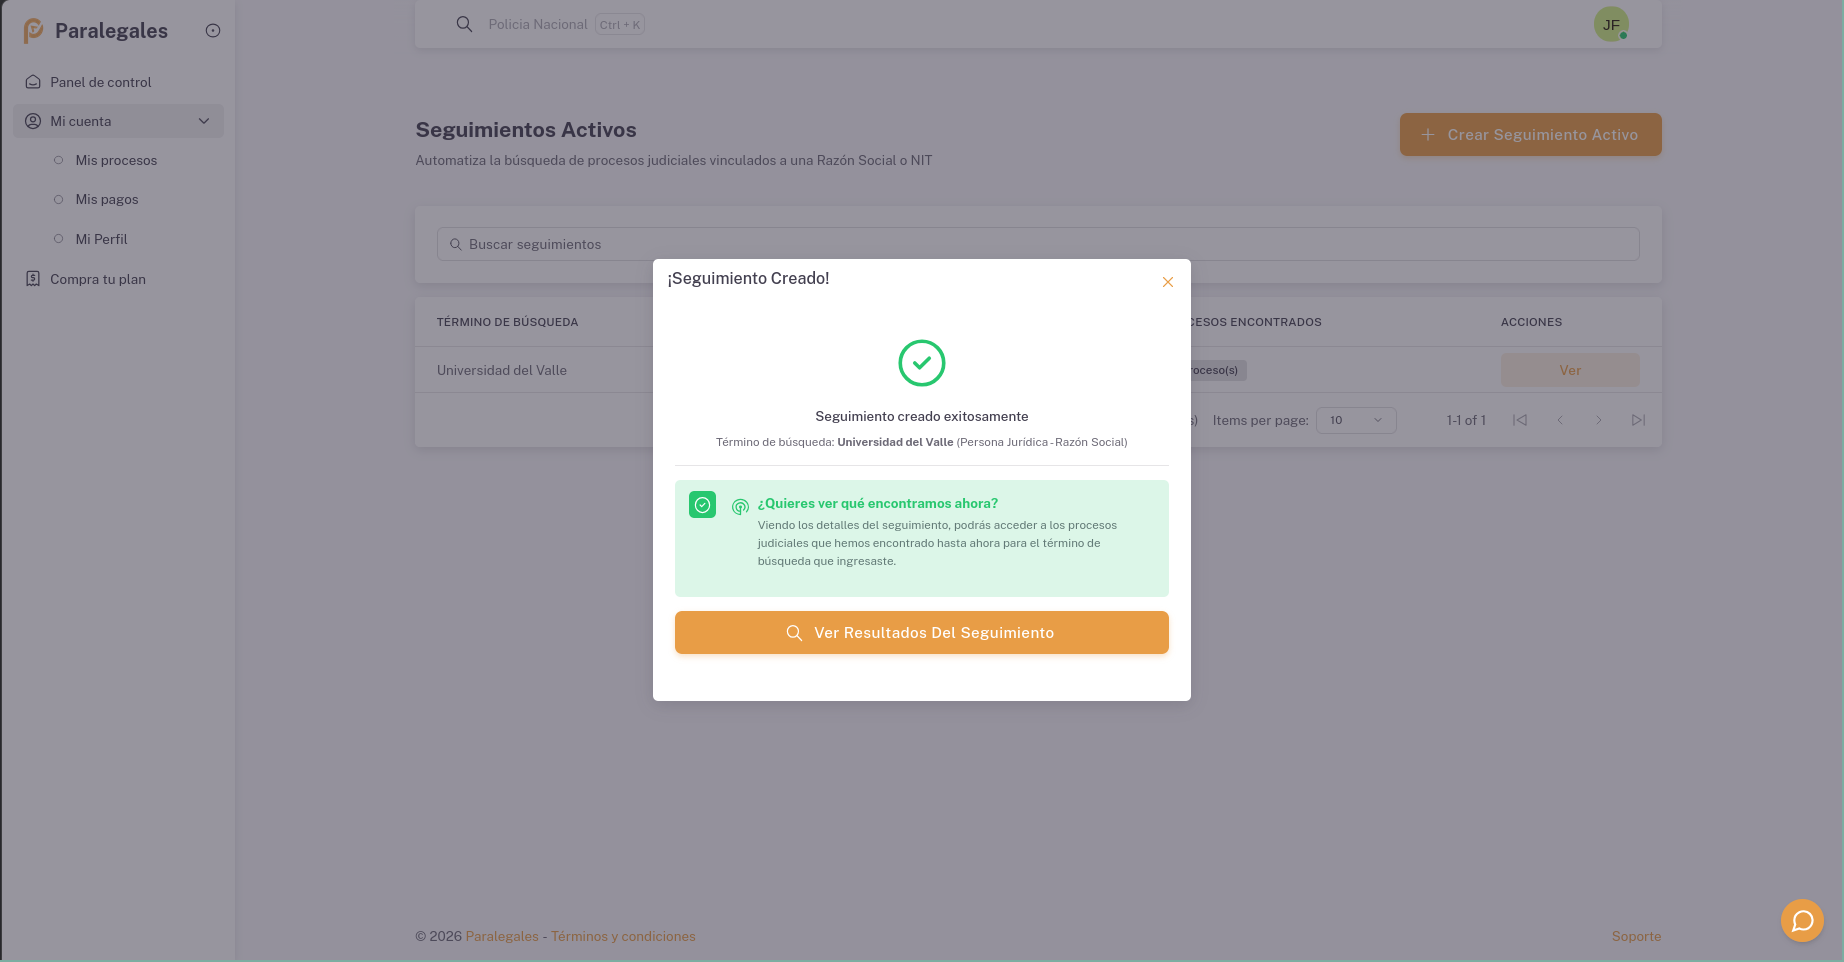
\includegraphics[width=1\textwidth]{img/figures/fig28-seguimiento-activo-success.png}
  \caption[\seguimientoActivoSuccessCaption]{\seguimientoActivoSuccessCaption Fuente: Elaboración propia.}
  \label{fig:seguimiento-activo-success}
\end{figure}

\subsubsection{Importación Masiva de Procesos}

Pensando en la usabilidad para nuevos despachos de abogados o equipos jurídicos con volúmenes considerables de casos, se implementó una funcionalidad de importación masiva que permite la carga simultánea de múltiples procesos en una sola operación.

Esta funcionalidad integra los módulos previamente descritos: recibe un conjunto de datos estructurado por parte del usuario y lo procesa de forma iterativa o por lotes en el \textit{backend}. El sistema verifica la existencia de cada proceso, valida los parámetros y ejecuta la lógica de seguimiento de forma individual, proporcionando al final un reporte sobre el estado de la importación. Esta operación optimiza drásticamente el tiempo operativo en comparación con el registro manual proceso por proceso, reduciendo la fricción inicial para equipos con carteras de casos de gran volumen. Complementando la operación orientada al usuario final, el siguiente módulo habilita la comunicación proactiva desde el portal administrativo, a través de campañas de mensajería masiva.

\subsection{Módulo de Campañas y Comunicación Masiva}\label{subsec:campanas}

El Módulo de Campañas fue diseñado para dotar a los operadores de la plataforma de una herramienta centralizada y eficiente para la captación, fidelización y comunicación directa con clientes potenciales. El módulo orquesta la gestión de información de contacto y facilita el envío proactivo de mensajes a través de múltiples canales. Su implementación abarcó tanto el diseño de la interfaz de administración como la construcción de la arquitectura \textit{backend} orientada al procesamiento de altos volúmenes de envíos.

\subsubsection{Interfaz de Administración y Experiencia de Usuario}

Para el portal administrativo, se implementó un conjunto de vistas interactivas destinadas al control completo sobre las operaciones de comunicación. La interfaz central del módulo ofrece una visualización tabular y estructurada donde los administradores pueden ejecutar el ciclo completo de gestión —creación, lectura, actualización y eliminación— sobre las campañas registradas. La \autoref{fig:campaigns-table} ilustra esta vista principal, donde cada fila de la tabla corresponde a una campaña con sus indicadores de estado, canal de envío y métricas de alcance, proporcionando una visión operativa integral al administrador.

\newcommand\campaignsTableCaption{Vista principal del módulo de campañas con listado tabular y operaciones CRUD sobre los registros. \hspace{1em}}
\begin{figure}[H]
  \centering
  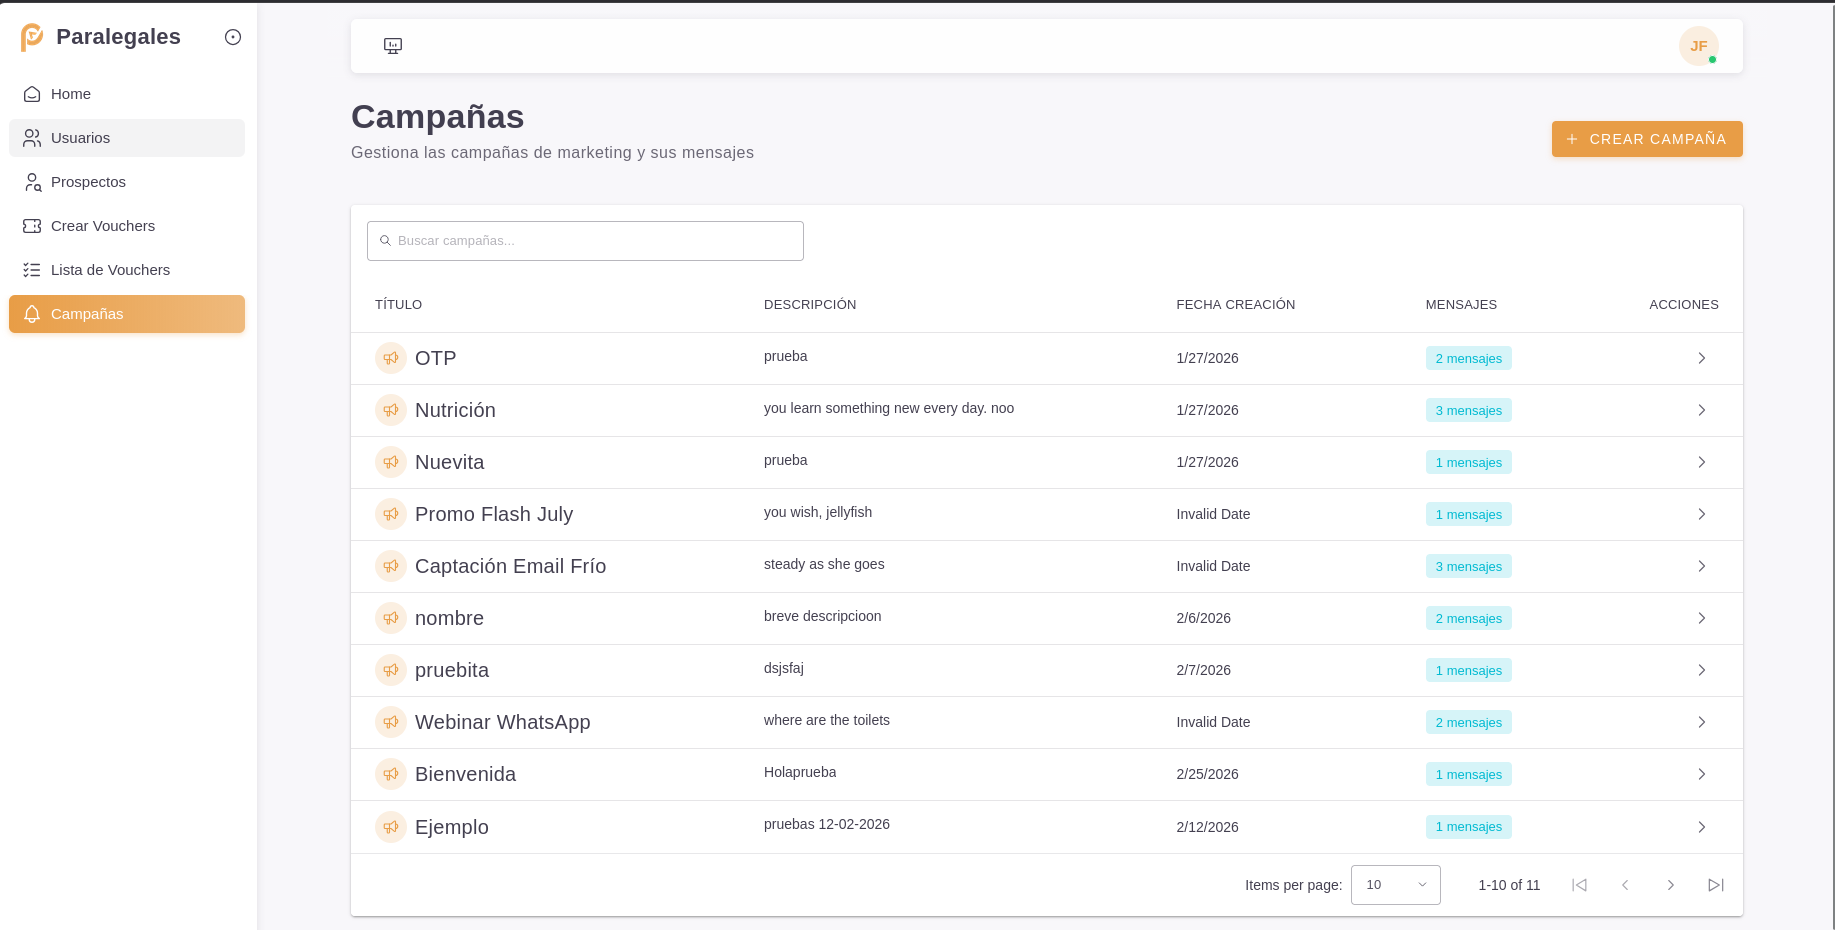
\includegraphics[width=1\textwidth]{img/figures/fig29-campaings-table.png}
  \caption[\campaignsTableCaption]{\campaignsTableCaption Fuente: Elaboración propia.}
  \label{fig:campaigns-table}
\end{figure}

Con el objetivo de maximizar la productividad y minimizar la fricción durante la navegación, se desarrolló un sistema de paneles laterales contextuales (\textit{sidebars}) que permite configurar los parámetros de envío, redactar mensajes y previsualizar el contenido sin abandonar la vista principal.

Adicionalmente, se diseñaron cuadros de diálogo especializados para ejecutar operaciones sobre campañas individuales. La \autoref{fig:editar-campana} presenta el formulario de edición de una campaña existente, que permite al administrador modificar sus atributos principales —nombre, descripción, canal y estado— desde un diálogo modal que preserva el contexto de la lista subyacente.

\newcommand\editarCampanaCaption{Diálogo de edición de una campaña existente con formulario de actualización de atributos principales. \hspace{1em}}
\begin{figure}[H]
  \centering
  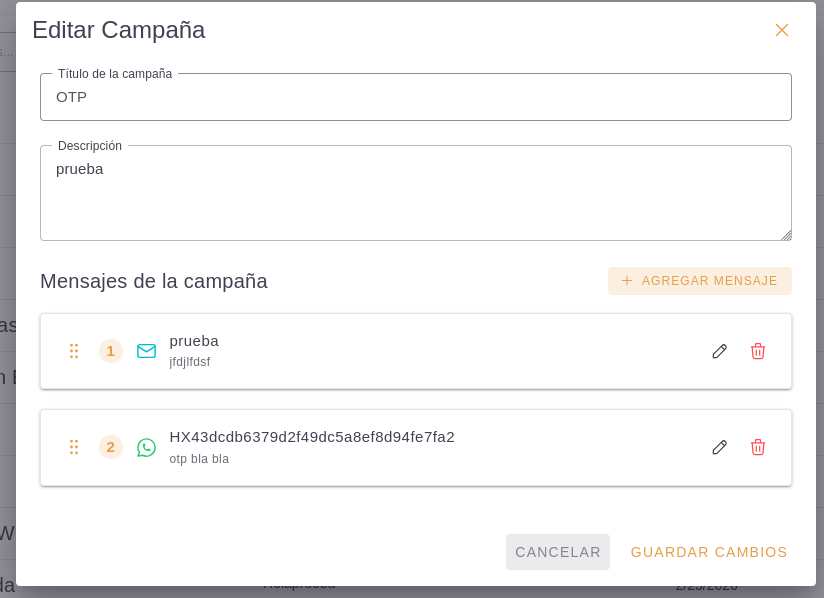
\includegraphics[width=0.85\textwidth]{img/figures/fig31-editar-campaing.png}
  \caption[\editarCampanaCaption]{\editarCampanaCaption Fuente: Elaboración propia.}
  \label{fig:editar-campana}
\end{figure}

Dentro de estos paneles, se incorporó una funcionalidad de plantillas dinámicas que permite insertar variables personalizadas —como el nombre del destinatario o detalles específicos de su caso—, las cuales son interpretadas y reemplazadas por el sistema en el momento del envío. La \autoref{fig:editar-mensaje} muestra el editor de contenido del mensaje, donde el administrador puede redactar el texto de la comunicación e insertar variables dinámicas mediante una interfaz asistida, con una previsualización del resultado final antes de ejecutar el envío masivo.

\newcommand\editarMensajeCaption{Editor de plantillas de mensaje con soporte para variables dinámicas personalizadas. \hspace{1em}}
\begin{figure}[H]
  \centering
  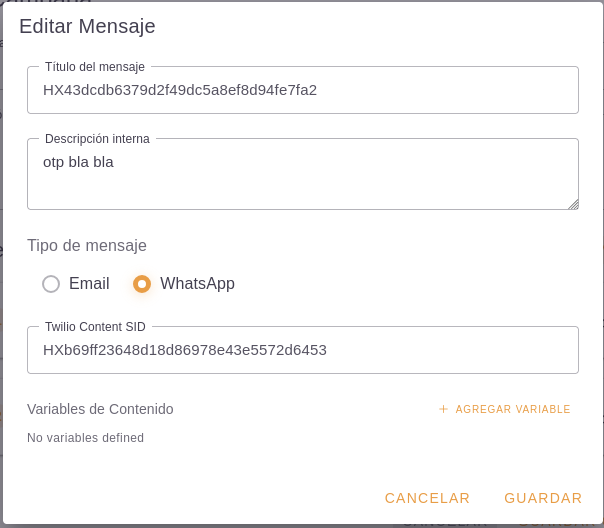
\includegraphics[width=0.85\textwidth]{img/figures/fig32-editar-msg.png}
  \caption[\editarMensajeCaption]{\editarMensajeCaption Fuente: Elaboración propia.}
  \label{fig:editar-mensaje}
\end{figure}

A nivel estructural en el \textit{frontend}, el módulo fue construido bajo un paradigma de componentes modulares y reutilizables, separando la presentación de la lógica de negocio. Se establecieron modelos estrictos de información para representar las entidades de campañas y clientes potenciales, complementados con un sistema de gestión de estado global que sincroniza reactivamente las interacciones del administrador con la base de datos documental en tiempo real, garantizando que cualquier modificación en los parámetros de una campaña se refleje de forma instantánea en todas las vistas de la plataforma.

\subsubsection{Procesamiento \textit{Backend} y Orquestación de Envíos Masivos}

El principal desafío técnico del módulo residía en la capacidad del sistema para procesar altos volúmenes de envíos sin degradar el rendimiento de la aplicación cliente ni incurrir en tiempos de espera prolongados (\textit{timeouts}). Para resolver esto, se diseñó e implementó una arquitectura \textit{backend} asíncrona basada en microservicios y funciones \textit{serverless}.

Cuando el administrador confirma un envío masivo desde el panel, el cliente transmite una solicitud estructurada hacia la nube. Esta petición es interceptada por una función bajo demanda que actúa como orquestadora: su responsabilidad principal no es enviar los mensajes de manera inmediata, sino validar la solicitud, desglosar el volumen total de destinatarios y depositar las instrucciones individuales de envío en el sistema de colas de mensajería SQS. Esta abstracción mediante colas desacopla por completo la experiencia del administrador de la latencia de red de los proveedores externos de mensajería. Posteriormente, otras funciones especializadas consumen estas colas, interpretan las variables dinámicas configuradas desde la interfaz y enrutan cada mensaje hacia el proveedor correspondiente —como servicios de correo electrónico o plataformas de mensajería instantánea—.

Para garantizar la fiabilidad técnica de la operación, se integraron capas de observabilidad y registro de eventos en cada punto del ciclo de vida del mensaje, permitiendo trazar el estado de una comunicación desde su origen en el panel de administración, su paso por el sistema de colas, hasta su entrega final. Esta arquitectura asíncrona constituye, de hecho, uno de los casos de uso más representativos del sistema de observabilidad transversal que se describe en el siguiente apartado.

\subsection{Sistema de Observabilidad y Telemetría}\label{subsec:observabilidad}

La diversidad de flujos que componen Paralegales —síncronos y asíncronos, internos y dependientes de proveedores externos— exige un sistema transversal capaz de registrar, correlacionar y exponer el comportamiento del sistema en producción. Para atender esta necesidad, se conceptualizó e implementó un subsistema de observabilidad estructurada y telemetría que monitorea las integraciones de red con proveedores fundamentales, como los servicios de la Rama Judicial y la plataforma Samai del Consejo de Estado. El sistema opera de forma transversal, capturando eventos tanto en el BFF construido con Nuxt en el lado del servidor, como en la arquitectura de microservicios de \textit{backend} desplegados mediante AWS Lambda y programados en Go.

\subsubsection{Arquitectura e Implementación}

En arquitecturas de microservicios, una única acción desencadenada por el usuario puede atravesar múltiples componentes, redes y servicios distribuidos antes de retornar una respuesta. Esta naturaleza distribuida introduce complejidad al momento de diagnosticar fallos, identificar cuellos de botella o auditar interrupciones del servicio. Para abordar este desafío, la observabilidad se consolidó como un pilar arquitectónico del sistema, aprovechando la correlación de registros (\textit{logs}), métricas y trazas para deducir el estado interno del sistema a partir de sus salidas externas.

Para garantizar la consistencia de los datos de telemetría, el sistema evita la inyección manual y aislada de registros en cada punto de conexión. En su lugar, emplea el patrón de clientes HTTP interceptores (\textit{Intercepting HTTP Clients}) que generan telemetría unificada de forma transparente:

\begin{itemize}
  \item \textbf{Capa de \textit{backend} (Go):} se desarrolló una envoltura sobre el cliente HTTP nativo que emite eventos estructurados por cada salto de red (inicio de la petición, finalización o error). Mediante contextos del lenguaje (\texttt{context.WithValue}), se inyectan metadatos vitales a los registros de forma segura y propagada, tales como el nombre del servicio, el entorno de ejecución, la operación en curso y los identificadores de trazabilidad (ID de solicitud e ID de correlación).

  \item \textbf{Capa de \textit{frontend} (BFF en Nuxt):} se implementaron interceptores sobre la utilidad nativa de consumo de APIs. Mediante \textit{middlewares}, se extrae la información de la sesión del usuario para enriquecer la telemetría. Adicionalmente, se integraron mecanismos de saneamiento (\textit{sanitizers}) que garantizan que ninguna información confidencial —como contraseñas o \textit{tokens} de autorización— se filtre a los registros de texto.
\end{itemize}

Ambas capas convergen en un modelo de esquema estandarizado que emite eventos en formato JSON puro. Este sobre de datos unifica la estructura de los registros de toda la aplicación, eliminando ambigüedades y facilitando su indexación automática en la infraestructura de la nube.

\subsubsection{Infraestructura en la Nube y Monitoreo Proactivo}

El procesamiento y la visualización de la telemetría se encuentran completamente automatizados mediante Infraestructura como Código (IaC) a través de AWS CloudFormation. Esta infraestructura transforma los registros en bruto en conocimiento técnico accionable mediante cuatro mecanismos complementarios:

\begin{itemize}
  \item \textbf{Filtros de métricas deducidas:} el sistema analiza en tiempo real las cargas útiles JSON para derivar métricas operativas sin instrumentación de código adicional. Se capturan indicadores como el volumen total de tráfico (número de solicitudes), la tasa de errores de servidor (códigos HTTP 5xx) y las fluctuaciones en la latencia.

  \item \textbf{Alertas y matemáticas de métricas:} se configuraron alarmas agregadas que vigilan el comportamiento global de los microservicios. Mediante el análisis de percentiles (como el p95 para medir el peor caso de latencia) y sumatorias en ventanas de tiempo de cinco minutos, el sistema detecta degradaciones significativas del servicio de forma automática.

  \item \textbf{Notificaciones en tiempo real:} ante la activación de una anomalía, el sistema desencadena un flujo automatizado hacia un tópico SNS que invoca una función Lambda especializada. Esta función analiza las condiciones del fallo y transmite instantáneamente una notificación enriquecida al equipo de desarrollo a través de un canal de Telegram.

  \item \textbf{Panel de control centralizado:} la infraestructura despliega automáticamente un tablero de control (\textit{dashboard}) interactivo que consolida gráficos de series de tiempo y herramientas de análisis relacional (\textit{Logs Insights}), permitiendo ejecutar consultas estructuradas para identificar rápidamente la causa raíz de un error masivo.
\end{itemize}

La \autoref{fig:dashboard-observabilidad} muestra el panel de control de CloudWatch generado por la infraestructura, donde los gráficos de series de tiempo visualizan en tiempo real el volumen de peticiones, la tasa de errores y la distribución de latencias por servicio. La \autoref{fig:dashboard-observabilidad-alerts} complementa este panorama con la vista de alarmas configuradas, donde cada indicador refleja su estado actual —en alerta, en recuperación o saludable— de forma inmediatamente legible para el equipo de ingeniería.

\newcommand\dashboardObservabilidadCaption{Panel de control de CloudWatch con métricas de tráfico, errores y latencia de los microservicios. \hspace{1em}}
\begin{figure}[H]
  \centering
  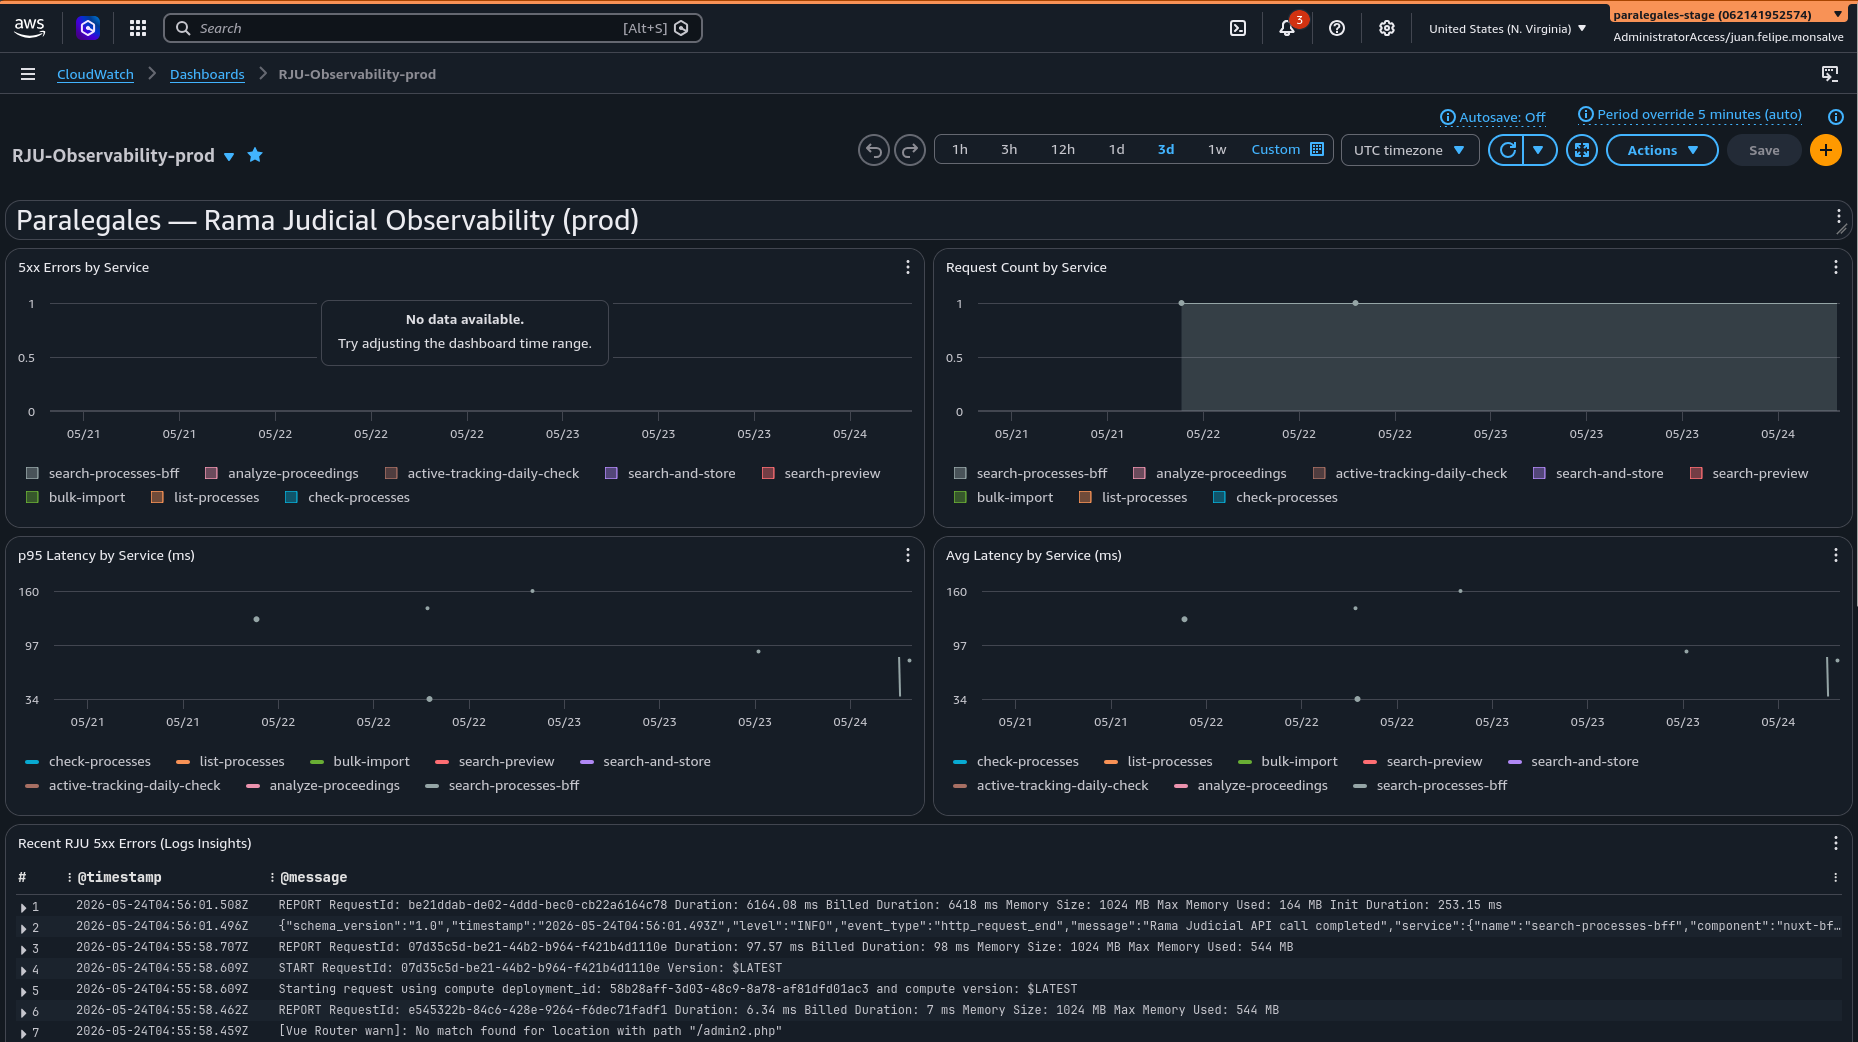
\includegraphics[width=1\textwidth]{img/figures/fig33-dashboard-observabilidad.png}
  \caption[\dashboardObservabilidadCaption]{\dashboardObservabilidadCaption Fuente: Elaboración propia.}
  \label{fig:dashboard-observabilidad}
\end{figure}

\newcommand\dashboardObservabilidadAlertsCaption{Vista de alarmas activas en CloudWatch con indicadores de estado por servicio monitoreado. \hspace{1em}}
\begin{figure}[H]
  \centering
  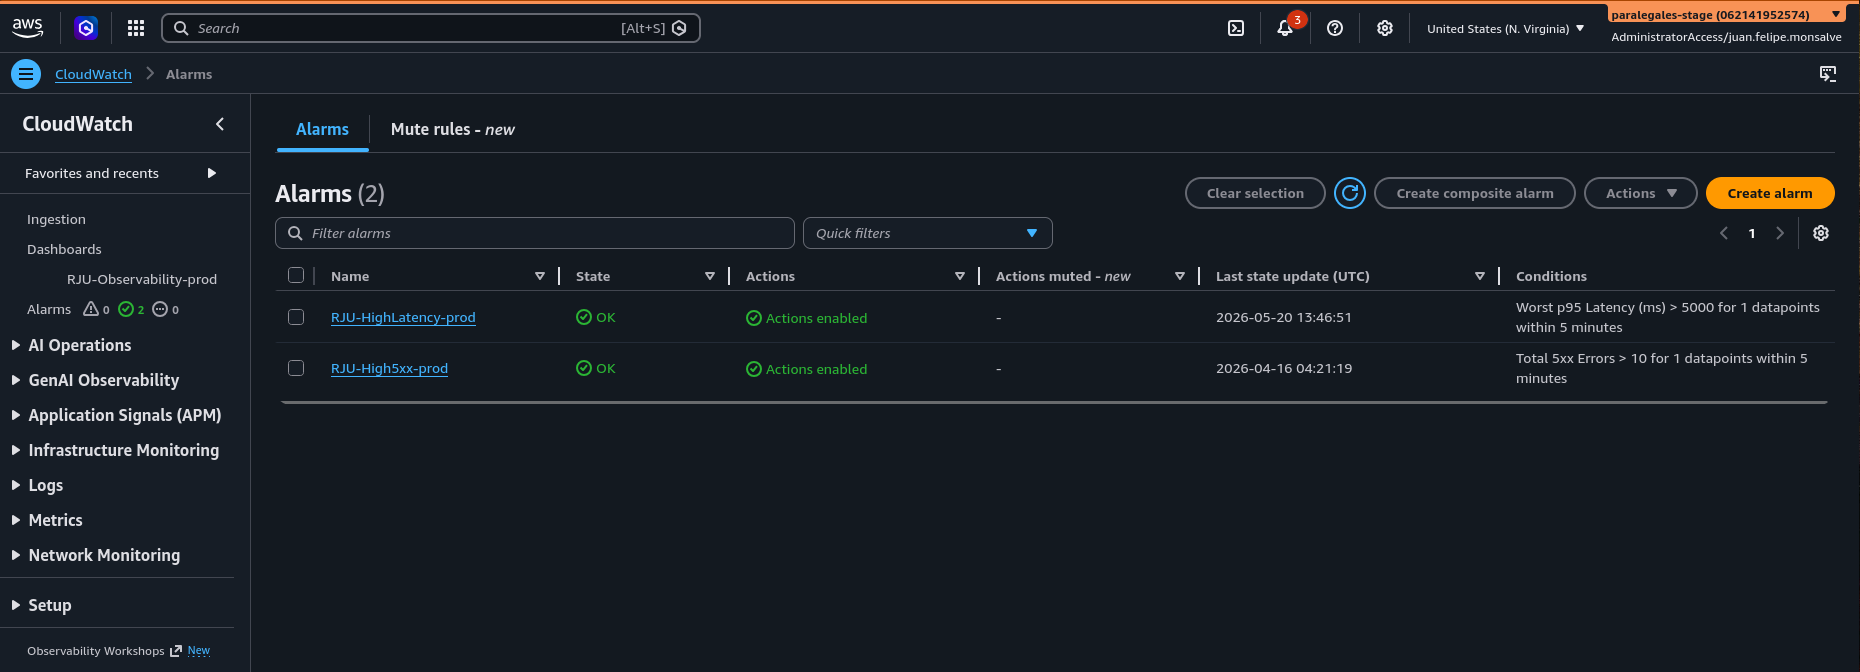
\includegraphics[width=1\textwidth]{img/figures/fig34-dashboard-observabilidad-alerts.png}
  \caption[\dashboardObservabilidadAlertsCaption]{\dashboardObservabilidadAlertsCaption Fuente: Elaboración propia.}
  \label{fig:dashboard-observabilidad-alerts}
\end{figure}

\newcommand\telegramAlertsObservabilityCaption{Canal de Telegram utilizado para la recepción de alertas automáticas del sistema. \hspace{1em}}
\begin{figure}[H]
  \centering
  \includegraphics[width=0.72\textwidth]{img/figures/fig13-telegram.png}
  \caption[\telegramAlertsObservabilityCaption]{\telegramAlertsObservabilityCaption Fuente: Elaboración propia.}
  \label{fig:telegram-alerts-observability}
\end{figure}

El impacto de este subsistema sobre la operación de la plataforma —la medición objetiva de la disponibilidad de los proveedores externos y la trazabilidad de errores por usuario— se valora como resultado del proyecto en el \autoref{subsec:resultado-c}.

Así como la observabilidad protege el sistema en su estado de operación continua, las prácticas que se describen a continuación resguardan la integridad y la calidad del código a lo largo de su proceso de evolución.

\subsection{Prácticas de Ciclo de Vida de Desarrollo y Aseguramiento de Calidad}\label{subsec:sdlc}

Para garantizar la estabilidad, la mantenibilidad y la evolución segura del ecosistema Paralegales, se implementó un conjunto riguroso de prácticas de ingeniería de software a lo largo del ciclo de vida de desarrollo (\textit{Software Development Life Cycle}, SDLC). Estas prácticas abarcan desde la estandarización del código en los entornos locales de los desarrolladores hasta la validación automática en los repositorios compartidos, conformando un sistema de aseguramiento de calidad continuo y multicapa.

\subsubsection{Estandarización de Código y \textit{Hooks} de Pre-commit}

Con el objetivo de mantener una base de código coherente y libre de errores sintácticos o de estilo, se integraron herramientas de análisis estático y formateo. El ecosistema utiliza ESLint para el \textit{linting} de archivos JavaScript, TypeScript y componentes Vue, y Prettier para el formateo estandarizado y uniforme de múltiples extensiones (incluyendo CSS, JSON, YAML y Markdown).

Para automatizar y hacer obligatorio el cumplimiento de estas reglas antes de que el código ingrese al control de versiones, se adoptó Lefthook como gestor de \textit{hooks} de Git. Su configuración define tres flujos de interceptación clave:

\begin{itemize}
  \item \textbf{\textit{Pre-commit}:} ejecuta en paralelo el formateo (\texttt{prettier --write}) y la validación estática (\texttt{eslint}) exclusivamente sobre los archivos que están en el área de preparación (\textit{staged files}). Si el código es formateado automáticamente, Lefthook lo re-agrega al \textit{commit} sin interrumpir el flujo de trabajo del desarrollador.

  \item \textbf{\textit{Commit-msg}:} garantiza la trazabilidad e historial semántico del proyecto aplicando el estándar \textit{Conventional Commits}. Mediante la integración de Commitlint, cada mensaje de \textit{commit} es evaluado para confirmar que cuenta con una estructura válida (tipo de cambio, alcance y descripción) y que respeta las longitudes máximas configuradas para garantizar legibilidad.

  \item \textbf{\textit{Post-merge}:} detecta si hubo cambios estructurales en el árbol de dependencias (modificaciones en \texttt{pnpm-lock.yaml} o \texttt{package.json}) tras una sincronización o fusión de ramas. Si es el caso, dispara automáticamente la instalación de paquetes (\texttt{pnpm install}) para mantener el entorno local perfectamente sincronizado.
\end{itemize}

\subsubsection{Integración Continua}

Las pipelines de integración continua (\textit{Continuous Integration}, CI) están orquestadas de manera declarativa a través de GitHub Actions. El flujo principal de integración (\texttt{ci.yml}) está diseñado para ejecutarse de forma obligatoria frente a (\textit{Pull Requests}) dirigidas a ramas protegidas, realizando validaciones estrictas con tiempos de procesamiento optimizados:

\begin{itemize}
  \item \textbf{Configuración de entorno y caché:} el \textit{pipeline} aprovisiona contenedores con Node.js e instala eficientemente las dependencias utilizando \texttt{pnpm}, apoyándose en el sistema de caché nativo de GitHub para reutilizar los módulos descargados en ejecuciones previas y reducir la duración total del proceso.

  \item \textbf{Validación diferencial:} se utilizan acciones especializadas de detección de cambios para ejecutar el \textit{linting} y las pruebas de formato únicamente sobre el subconjunto de archivos que sufrieron modificaciones reales, evitando análisis innecesarios sobre código sin cambios.
\end{itemize}

\subsubsection{Estrategia de Pruebas Automatizadas}

La confiabilidad funcional y el blindaje de los datos se soportan en una estrategia de pruebas centrada en la validación de las reglas de seguridad, apoyada en la Firebase Emulator Suite para ejecutar las pruebas en un entorno local y efímero sin afectar entornos reales. Esta estrategia, junto con la validación manual sistemática sobre el entorno de \textit{staging} y la evaluación de pruebas \textit{end-to-end}, se aborda de forma dedicada en el capítulo de pruebas del sistema, por lo que aquí se la referencia sin reproducir su detalle.

La integración de estas prácticas a lo largo del SDLC —desde el \textit{commit} inicial hasta la ejecución del \textit{pipeline} de CI— configura un sistema de aseguramiento de calidad que opera de forma continua y automatizada, reduciendo el riesgo de regresiones y garantizando que cada iteración del sistema mantenga los estándares de calidad y seguridad establecidos para la plataforma.

